
%卒業論文用雛形
%\documentclass[a4j,12pt,oneside,openany]{jsbook}
% 英語なら以下を使う.
\documentclass[a4j,12pt,oneside,openany,english,dvipdfmx]{jsbook}

\usepackage{amsfonts,amsmath,amssymb}
\usepackage{bm}
\usepackage{float}
\usepackage[dvipdfmx]{graphicx}
\usepackage{color}
%\usepackage[dvipdfmx]{hyperref}
\usepackage{algorithm}
\usepackage{algorithmic}
%\usepackage{txfonts}
%\usepackage{ascmac, here}
\usepackage{listings}
\usepackage{color}
%\usepackage{url}
\usepackage{comment}

%jsbook を report っぽくするスタイルファイル
\usepackage{book2report}
%定理,補題,系,例題,証明などや英語用の定義がされています.
%自分なりにいじってください.
\usepackage{thesis}
% 具体的には以下のように定義されています.
% 英語の定理環境
%  \newtheorem{theorem}{Theorem}[chapter]
%  \newtheorem{lemma}{Lemma}[chapter]
%  \newtheorem{proposition}{Proposition}[chapter]
%  \newtheorem{corollary}{Corollary}[chapter]
%  \newtheorem{definition}{Definition}[chapter]
%  \newtheorem{example}{Example}[chapter]
%  \newtheorem{proof}{Proof}
% 日本語の定理環境
%  \newtheorem{theorem}{定理}[chapter]
%  \newtheorem{lemma}{補題}[chapter]
%  \newtheorem{proposition}{命題}[chapter]
%  \newtheorem{corollary}{系}[chapter]
%  \newtheorem{definition}{定義}[chapter]
%  \newtheorem{example}{例}[chapter]
%  \newtheorem{proof}{証明}
% 証明には番号をつけず,最後は Box で終わります.

\allowdisplaybreaks[1]

\newcommand{\mysps}{\ensuremath{[\![s^{\otimes}]\!]}_s}
\newcommand{\myspq}{\ensuremath{[\![s^{\otimes}]\!]}_q}
\newcommand{\myspds}{\ensuremath{[\![s^{\otimes \prime}]\!]}_s}
\newcommand{\myspdq}{\ensuremath{[\![s^{\otimes \prime}]\!]}_q}
\newcommand{\argmax}{\mathop{\rm arg~max}\limits}
\newcommand{\argmin}{\mathop{\rm arg~min}\limits}

% 英語で,見出しのフォントが気に入らなかったら
\renewcommand{\headfont}{\bfseries}

%ページ数が少ないときはここを大きくしてごまかそう!!効果絶大!!
\renewcommand{\baselinestretch}{1.1}

\begin{document}
%%%%%%%%%%%% 題目 %%%%%%%%%%%%%%%%%%%%%%%%%%%%%%%%%%%%%%%%%%%%%%%%%%%%%%%
%%%%%%%%%%%% ここも適当に変えてもいいと思う %%%%%%%%%%%%%%%%%%%%%%%%%%%%%%%%%
\thispagestyle{empty}
\begin{center}
\vspace*{5mm}
{\Huge {\bf 特 \hspace{12pt} 別 \hspace{12pt} 研 \hspace{12pt} 究 \hspace{12pt} 報 \hspace{12pt} 告}}\\
\vspace{2cm}
{\Large 題\hspace{8mm}目}\\
\vspace{1cm}
\underline{\LARGE{This Is}} \\
\vspace{0.5cm}
\underline{\LARGE{My Bachelor Thesis}} \\
\vspace{12mm}
{\large 指 導 教 員}\\
\vspace{6mm}
\underline{\Large Professor Jane Doe}\\
 \\
\underline{\Large Associate Professor Joe Smith}\\
\vspace{8mm}
{\large 報 告 者}\\
\vspace{6mm}
\underline{\Large John Doe}\\
\vspace{10mm}
{\Large 平成28年2月吉日}\\
\vspace{14mm}
{\Large 大阪大学基礎工学部システム科学科\\知能システム学コース}\\
\end{center}
\clearpage
\setcounter{page}{0}
\pagenumbering{roman}

%%%%%%%%%%%% 概要 %%%%%%%%%%%%%%%%%%%%%%%%%%%%%%%%%%%%%%%%%%%%%%%%%%%%
\begin{abstract}
  This is abstruct.
\end{abstract}


%%%%%%%%%%%% 目次 %%%%%%%%%%%%%%%%%%%%%%%%%%%%%%%%%%%%%%%%%%%%%%%%%%%%
\clearpage
\tableofcontents
\clearpage
\setcounter{page}{0}
\pagenumbering{arabic}

%%%%%%%%%%%% 1章 %%%%%%%%%%%%%%%%%%%%%%%%%%%%%%%%%%%%%%%%%%%%%%%%%%%
\chapter{Introduction}
Test of Theorem.

\section{First of All}

\begin{theorem}[First Theorem]
This is Theorem.
\end{theorem}

\begin{lemma}[First Lemma]
This is Lemma.
\end{lemma}

\begin{proposition}[First Proposition]
This is Proposition.
\end{proposition}

\begin{corollary}[First Corollary]
This is Corollary.
\end{corollary}

\begin{proof}
This is true, obviously.
\end{proof}

\begin{definition}[First Definition]
We call this ``That''.
\end{definition}

\begin{example}[First Example]
This is an example.
\end{example}

\section{Next of First of All}
\subsection{First Subsection}
\subsubsection{First Subsubsection}

Test of Equation.
\begin{equation}
	a = b + c
\end{equation}

\begin{table}
	\caption{Test of Table Caption}
\end{table}

\begin{figure}
	\caption{Test of Figure Caption}
\end{figure}


%%%%%%%%%%%% 2nd Chapter %%%%%%%%%%%%%%%%%%%%%%%%%%%%%%%%%%%%%%%%%%%%%%%%%%%
\chapter{2nd Chapter}

\section{Markov Decision Processes and Reinforcement Learning}

\begin{definition}[Labeled Markov Decision Process]
A (labeled) Markov decision process (MDP) is a tuple $M$ = $(S, A, \mathcal{A}, P, s_{init}, AP, L)$, where S is a finite set of states, $A$ is a finite set of actions, $\mathcal{A} : S \rightarrow 2^A$ is a mapping that maps each state to the set of possible actions at the state, $P:S \times S \times A \rightarrow [0,1]$ is a transition probability such that $\sum_{s' \in S} P(s'|s,a) = 1$ for any state $s \in S$ and any action $a \in \mathcal{A}(s) $, $s_{init} \in S$ is the initial state, $AP$ is a finite set of atomic propositions, and $L : S \times A \times S\ \rightarrow\ 2^{AP}$ is a labeling function that assigns a set of atomic propositions to each transition $(s, a, s') \in S \times A \times S$.

In the MDP $M$, an infinite path starting from a state $s_0 \in S$ is defined as a sequence $\rho\ =\ s_0a_0s_1 \ldots\ \in S (A S)^{\omega}$ such that $P(s_{i+1}|s_i, a_i) > 0$ for any $ i \in \mathbb{N}_0$, where $\mathbb{N}_0$ is the set of natural numbers including zero.  A finite path is a finite sequence in $S (A S)^*$. In addition, we sometimes represent $\rho$ as $\rho_{init}$ to emphasize that $\rho$ starts from $s_0 = s_{init}$.
For a path $\rho\ =\ s_0a_0s_1 \ldots$, we define the corresponding labeled path $L(\rho)\ =\ L(s_0,a_0,s_1)L(s_1,a_1,s_2) \ldots \in (2^{AP})^{\omega}$. $InfPath^{M}\ ( \text{resp., }FinPath^{M})$ is defined as the set of infinite (resp., finite) paths starting from $s_0=s_{init}$ in the MDP $M$. For each finite path $\rho$, $last(\rho)$ denotes its last state.
\label{MDP}
\end{definition}

\begin{definition}[Policy]
  A policy on an MDP $M$ is defined as a mapping $\pi:FinPath^{M} \times \mathcal{A}(last(\rho)) \rightarrow [0,1]$. A policy $\pi$ is a {\it positional} policy if for any $ \rho \in FinPath^{M}$ and any $ a \in \mathcal{A}(last(\rho))$, it holds that $\pi(\rho, a)=\pi(last(\rho),a)$ and there exists $ a' \in \mathcal{A}(last(\rho))$ such that
  \begin{align*}
    \pi(\rho, a) =
    \left\{
    \begin{aligned}
      1 &   & &\text{if}\ a=a',\\
      0 &   & &\text{otherwise}.
    \end{aligned}
    \right.
  \end{align*}
\end{definition}

Let $InfPath^{M}_{\pi}$ (resp., $FinPath^{M}_{\pi}$) be the set of infinite (resp., finite) paths starting from $s_0=s_{init}$ in the MDP $M$ under a policy $\pi$. The behavior of an MDP $M$ under a policy $\pi$ is defined on a probability space $(InfPath^{M}_{\pi}, \mathcal{F}_{InfPath^{M}_{\pi}}, Pr^{M}_{\pi})$. % over the set of infinite paths $InfPath^{M}_{\pi}$ on the MDP $M$ with the policy $\pi$.

\begin{definition}[Markov chain]
  A Markov chain induced by an MDP $M$ with a positional policy $\pi$ is a tuple $MC_{\pi} = (S_{\pi},P_{\pi},s_0,AP,L)$, where $S_{\pi} = S$, $P_{\pi}(s'|s) = P(s'|s,a)$ for $s, s^{\prime} \in S$ and $a \in \mathcal{A}(s)$ such that $\pi(s,a) = 1$.
  The state set $S_{\pi}$ of $MC_{\pi}$ can be represented as a disjoint union of a set of transient states $T_{\pi}$ and closed irreducible sets of recurrent states $R^j_{\pi}$ with $j \in \{ 1, \ldots ,h \}$, as $ S_{\pi} = T_{\pi} \sqcup R^1_{\pi} \sqcup \ldots \sqcup R^h_{\pi} $ \cite{ESS}.
  In the following, we say a ``recurrent class'' instead of a ``closed irreducible set of recurrent states'' for simplicity.
\end{definition}

In an MDP $M$, we define a reward function $\mathcal{R}:S \times A \times S \rightarrow \mathbb{R}$, where $\mathbb{R}$ is the set of real numbers. The function denotes the immediate scalar bounded reward received after the agent performs an action $a$ at a state $s$ and reaches a next state $s'$ as a result.

\begin{definition}[Expected discounted reward for MDPs]
  For a policy $\pi$ on an MDP $M$, any state $s \in S$, and a reward function $\mathcal{R}$, we define the expected discounted reward as
  \begin{align*}
    V^{\pi}(s)= \mathbb{E}^{\pi}[\sum_{n=0}^{\infty}\gamma^n \mathcal{R}(S_n, A_n, S_{n+1})|S_0 = s],
  \end{align*}
where $\mathbb{E}^{\pi}$ denotes the expected value given that the agent follows the policy $\pi$ from the state $s$ and $\gamma \in [0,1)$ is a discount factor. Intuitively, the magnitude of the discount factor $\gamma$ determines how much we consider rewards received in the future. The function $V^{\pi}(s)$ is often referred to as a state-value function under the policy $\pi$. For any state-action pair $(s,a) \in S \times A$, we define an action-value function $Q^{\pi}(s,a)$ under the policy $\pi$ as follows.
  \begin{align*}
    Q^{\pi}(s,a)= \mathbb{E}^{\pi}[\sum_{n=0}^{\infty}\gamma^n \mathcal{R}(S_n, A_n, S_{n+1})|&S_0 = s, A_0 = a].
  \end{align*}

  We have the following recursively equation for the state-value function and the action-value function.

  \begin{align*}
    V^{\pi}(s) = & \mathbb{E}^{\pi}[\sum_{n=0}^{\infty}\gamma^n \mathcal{R}(S_n, A_n, S_{n+1})|S_0 = s] \\
     = & \sum_{a \in \mathcal{A}(s)} \pi(s,a) \sum_{s^{\prime} \in S} P(s^{\prime}|s,a) \mathbb{E}^{\pi}[\sum_{n=0}^{\infty}\gamma^n \mathcal{R}(S_n, A_n, S_{n+1})|S_0 = s, A_0 = a, S_1 = s^{\prime}] \\
     = & \sum_{a \in \mathcal{A}(s)} \pi(s,a) \sum_{s^{\prime} \in S} P(s^{\prime}|s,a) \{ \mathcal{R}(s, a, s^{\prime}) + \gamma \mathbb{E}^{\pi}[\sum_{n=0}^{\infty}\gamma^n \mathcal{R}(S_n, A_n, S_{n+1})|S_1 = s^{\prime}] \} \\
    = & \sum_{a \in \mathcal{A}(s)} \pi(s,a) \sum_{s^{\prime} \in S} P(s^{\prime}|s,a) \{ \mathcal{R}(s, a, s^{\prime}) + \gamma V^{\pi}(s^{\prime}) \},
  \end{align*}
\end{definition}

by the definition of the action-vlue function, it holds That

\begin{align*}
  Q^{\pi}(s,a) = & \max_{a \in \mathcal{A}(s)}V^{\pi}(s) \\
               = & \sum_{s^{\prime} \in S} P(s^{\prime}|s,a) \{ \mathcal{R}(s, a, s^{\prime}) + \gamma V^{\pi}(s^{\prime}) \} \\
               = & \sum_{s^{\prime} \in S} P(s^{\prime}|s,a) \{ \mathcal{R}(s, a, s^{\prime}) + \gamma \sum_{a^{\prime} \in \mathcal{A}(s^{\prime})} \pi(s^{\prime}, a^{\prime}) Q^{\pi}(s^{\prime},a^{\prime}) \}.
\end{align*}
 The above equations are called the {\it Bellman equation}.

\begin{definition}[Optimal policy]
  For any state $s$ in $S$, a policy $\pi^{\ast}$ is optimal if
  \begin{align*}
    \pi^{\ast} \in \argmax_{\pi \in \Pi^{pos}} V^{\pi}(s),
  \end{align*}
where $\Pi^{pos}$ is the set of positional policies over the state set $S$.

We have the following {\it Bellman optimality functions} by the optimal policy.

\begin{align*}
  V^{\pi^{\ast}}(s) = & \max_{\pi \in \Pi^{pos}} V^{\pi}(s) \\
                    = & \max_{\pi \in \Pi^{pos}} \sum_{a \in \mathcal{A}(s)} \pi(s,a) \sum_{s^{\prime} \in S} P(s^{\prime}|s,a) \{ \mathcal{R}(s, a, s^{\prime}) + \gamma V^{\pi}(s^{\prime}) \} \\
                    = & \max_{a \in \mathcal{A}(s)} [ \sum_{s^{\prime} \in S} P(s^{\prime}|s,a) \{ \mathcal{R}(s, a, s^{\prime}) + \gamma V^{\pi^{\ast}}(s^{\prime}) \} ],
\end{align*}

\begin{align*}
  Q^{\pi^{\ast}}(s,a) = & \max_{\pi \in \Pi^{pos}} Q^{\pi}(s,a) \\
                      = & \max_{\pi \in \Pi^{pos}} \sum_{s^{\prime} \in S} P(s^{\prime}|s,a) \{ \mathcal{R}(s, a, s^{\prime}) + \gamma \sum_{a^{\prime} \in \mathcal{A}(s^{\prime})} \pi(s^{\prime}, a^{\prime}) Q^{\pi}(s^{\prime},a^{\prime}) \} \\
                      = & \sum_{s^{\prime} \in S} P(s^{\prime}|s,a) \{ \mathcal{R}(s, a, s^{\prime}) + \gamma \max_{\pi \in \Pi^{pos}} \sum_{a^{\prime} \in \mathcal{A}(s^{\prime})} \pi(s^{\prime}, a^{\prime}) Q^{\pi}(s^{\prime},a^{\prime}) \} \\
                      = & \sum_{s^{\prime} \in S} P(s^{\prime}|s,a) \{ \mathcal{R}(s, a, s^{\prime}) + \gamma \max_{a \in \mathcal{A}(s^{\prime})} Q^{\pi}(s^{\prime},a^{\prime}) \}.
\end{align*}
\label{opt_pol}
\end{definition}

\section{Stochastic Discrete Event Systems}

\begin{definition}[Stochastic discrete event system]
We represent a stochastic discrete event system (DES) as a labeled Markov decision process (MDP). A DES is a tuple $D$ = $(S, E, \mathcal{E}, P_T, P_E, s_{init}, AP, L)$, where S is a finite set of states; $E$ is a finite set of events; $\mathcal{E} : S \rightarrow E$ is a mapping that maps each state to the set of feasible events at the state; $P_T:S \times S \times E \rightarrow [0,1]$ is a transition probability such that $\sum_{s' \in S} P_T(s'|s,e) = 1$ for any state $s \in S$ and any event $e \in \mathcal{E}(s) $ and $P_T(s'|s,e) = 0$ for any $e \notin \mathcal{E}(s)$; $P_E : E \times S \times 2^E \rightarrow [0,1]$ is the probability that an event occurs under a subset $\pi \in \mathcal{E}(s)$ of events allowed to occur at the state $s \in S$ such that $\Sigma_{e \in \pi} P_E(e|s,\pi) = 1$ and we call the subset the control pattern; for any $(s^{\prime}, s, \pi) \in S \times S \times 2^E$, we define the probability $P : S \times S \times 2^{E} \rightarrow [0,1]$ such that $P(s'|s,\pi) = \sum_{e \in \pi}P_E(e|s,\pi) P_T(s^{\prime}|s,e)$ and $\Sigma_{s^{\prime} \in S} P(s'|s,\pi) = 1$; $s_{init} \in S$ is the initial state; $AP$ is a finite set of atomic propositions; and $L : S \times E \times S \rightarrow 2^{AP}$ is a labeling function that assigns a set of atomic propositions to each transition $(s, e, s') \in S \times E \times S$. We assume that $E$ can be partitioned into the set of controllable events $E_c$ and the set of uncontrollable events $E_{uc}$ such that $E_c \cup E_{uc} = E$ and $E_c \cap E_{uc} = \emptyset$. Note that each event $e$ occurs probabilistically depending on only the current state and the subset of feasible events at the state given by a controller.

In the DES $D$, an infinite path for the DES starting from a state $s_0 \in S$ is defined as a sequence $\rho^D\ =\ s_0\pi_0e_0s_1 \ldots\ \in S (2^E E S)^{\omega}$ such that $P_E(e_i|s_i, \pi_i) > 0$ and $P_T(s_{i+1}|s_i, e_i) > 0$ for any $ i \in \mathbb{N}_0$. A finite path for the DES is a finite sequence in $S (2^E E S)^*$. In addition, we sometimes represent $\rho^D$ as $\rho^D_{init}$ to emphasize that $\rho^D$ starts from $s_0 = s_{init}$.
For a path $\rho^D\ =\ s_0\pi_0e_0s_1 \ldots$, we define the corresponding labeled path $L(\rho^D)\ =\ L(s_0,e_0,s_1)L(s_1,e_1,s_2) \ldots \in (2^{AP})^{\omega}$.
For simplicity, we often represent infinite (resp., finite) path for the DES as infinite (resp., finite) path and omit superscript $D$ of the paths.
% We define the set of finite labeled paths as $\mathcal{L}(M) = \{ L(\rho) \in (2^{AP})^{\omega} ; \rho = s_0e_0s_1 \ldots \in S(ES)^{\ast},\ P(s_{i+1}|s_i, e_i) > 0,\ i \in \mathbb{N}_0  \}.
 $InfPath^{D}\ ( \text{resp., }FinPath^{D})$ is defined as the set of infinite (resp., finite) paths starting from $s_0=s_{init}$ in the DES $D$. For each finite path $\rho$, $last(\rho)$ denotes its last state.
\end{definition}

We define the supervisor as a controller for the DES that restricts the behaviors of the DES to satisfy a given specification.

\begin{definition}[Supervisor]
For the DES $D$,  a supervisor $SV : FinPath^{D} \rightarrow 2^E$ is defined as a mapping that maps each finite path to a set of allowed events at the finite path and we call the set the control pattern. In the following, the supervisor we consider is {\it state-based}, namely for any $\rho \in FinPath^{D}$, $SV(\rho) = SV(last(\rho))$. Note that the relation $E_{uc} \subset SV(\rho) \subset E$ holds for any $\rho \in FinPath^D$.
Let $InfPath^{D}_{SV}$ (resp., $FinPath^{D}_{SV}$) be the set of infinite (resp., finite) paths starting from $s_0=s_{init}$ in the DES $D$ under a supervisor $SV$. The behavior of an DES $D$ under a supervisor $SV$ is defined on a probability space $(InfPath^{D}_{SV}, \mathcal{F}_{InfPath^{D}_{SV}}, Pr^{D}_{SV})$.
\end{definition}

We consider the objective function similar to the {\it Bellamn optimality function} defined by the definition \ref{opt_pol}.
\begin{definition}[Optimal value function for DESs]

  From the view point of reinforcement learning, the DES can be interpreted as the environment controlled by the supervisor and the supervisor can be interpreted as the policy. We introduce the two following assumptions.

  \begin{enumerate}
    \item The relative frequency of occurrence of each event does not depend on the control pattern.
    \item We define a reward function $\mathcal{R} : S \times 2^E \times E \times S \rightarrow \mathbb{R}$ and the reward $\mathcal{R}$ can be decomposed into $\mathcal{R}_1$ and $\mathcal{R}_2$. The first reward $\mathcal{R}_1 : S \times 2^E \rightarrow \mathbb{R}$ is determined by the control pattern selected by the supervisor, which depends on only the control pattern and the current state. The second reward $\mathcal{R}_2 : S \times E \times S \rightarrow \mathbb{R}$ is determined by the occurrence of an event and the corresponding state transition. For any $(s,\pi,e,s^{\prime}) \in S \times 2^E \times E \times S$, we then have
    \begin{align}
      \mathcal{R}(s,\pi,e,s^{\prime}) = \mathcal{R}_1(s,\pi) + \mathcal{R}_2(s,e,s^{\prime}).
    \end{align}
  \end{enumerate}
  Under the above assumptions, we have the following {\it Bellman optimality equation}.

  \begin{align}
    Q^{\ast}(s,\pi) = & \sum_{s^{\prime} \in S} P(s^{\prime}|s,\pi)\left \{ \mathcal{R}(s,\pi,e,s^{\prime}) + \gamma \max_{\pi^{\prime} \in 2^{\mathcal{E}(s^{\prime})}} Q^{\ast}(s^{\prime},\pi^{\prime}) \right \} \nonumber \\
    = & \sum_{s^{\prime} \in S} \sum_{e \in \pi} P_E(e|s,\pi) P_T(s^{\prime}|s,e) \left \{ \mathcal{R}_1(s,\pi) + \mathcal{R}_2(s,e,s^{\prime}) + \gamma \max_{\pi^{\prime} \in 2^{\mathcal{E}(s^{\prime})}} Q^{\ast}(s^{\prime},\pi^{\prime}) \right \} \nonumber \\
    = & \mathcal{R}_1(s,\pi) + \sum_{e \in \pi} P_E(e|s,\pi) \sum_{s^{\prime \in S}} P_T(s^{\prime}|s,e) \left \{ \mathcal{R}_2(s^{\prime}|s,e) + \gamma \max_{\pi^{\prime} \in 2^{\mathcal{E}(s^{\prime})}} Q^{\ast}(s^{\prime}, \pi^{\prime}) \right \},
  \end{align}
  where $\gamma \in [0,1)$.

  We introduce the following function. $T^{\ast} : S \times E \rightarrow \mathbb{R}$ such that
  \begin{align}
    T^{\ast}(s,e) = \sum_{s^{\prime \in S}} P_T(s^{\prime}|s,e) \left \{ \mathcal{R}_2(s^{\prime}|s,e) + \gamma \max_{\pi^{\prime} \in 2^{\mathcal{E}(s^{\prime})}} Q^{\ast}(s^{\prime}, \pi^{\prime}) \right \}.
  \end{align}
  We then have
  \begin{align}
    Q^{\ast}(s,\pi) = \mathcal{R}_1(s,\pi) + \sum_{e \in \pi}P_E(e|s,\pi) T^{\ast}(s,e).
  \end{align}

\end{definition}

\begin{definition}[Optimal supervisor]
We define an optimal supervisor $SV^{\ast}$ as follows. For any state $s \in S$,
\begin{align}
  SV^{\ast}(s) = \pi \in \argmax_{pi \in \mathcal{E}(s)} Q^{\ast}(s,\pi),
\end{align}
\end{definition}

\section{Linear Temporal Logic and Automata}

In our proposed method, we use linear temporal logic (LTL) formulas to describe various constraints or properties and to systematically assign corresponding rewards.
%For some complicated constraints, it is hard to assign such a corresponding reward function and to find a policy satisfying an LTL formula by the conventional reward assignments.
LTL formulas are constructed from a set of atomic propositions, Boolean operators, and temporal operators. We use the standard notations for the Boolean operators: $\top$ (true), $\neg$ (negation), and $\land$ (conjunction).
LTL formulas over a set of atomic propositions $AP$ are recursively defined as
\begin{align*}
  \varphi ::=\top\ |\ \alpha \in AP\ |\ \varphi_1 \land \varphi_2\ |\ \neg \varphi\ |\ \text{{\bf X}} \varphi\ |\ \varphi_1 \text{{\bf U}} \varphi_2,
\end{align*}
where $\varphi$, $\varphi_1$, and $\varphi_2$ are LTL formulas.
Additional Boolean operators are defined as $\perp := \neg \top $, $\varphi_1 \lor \varphi_2 := \neg(\neg \varphi_1 \land \neg \varphi)$, and $\varphi_1 \Rightarrow \varphi_2 := \neg \varphi_1 \lor \varphi_2$.
The operators {\bf X} and {\bf U} are called ``next" and ``until", respectively.
Using the operator {\bf U}, we define two temporal operators: (1) {\it eventually}, $\text{{\bf F}} \varphi := \top \text{{\bf U}} \varphi $ and (2) {\it always}, $\text{{\bf G}} \varphi := \neg \text{{\bf F}} \neg \varphi$.

Let $ M $ be an MDP.
For an infinite path $\rho = s_0a_0s_1 \ldots $ of $ M $ with $ s_0 \in S $, let $\rho[i]$ be the $i$-th state of $\rho$ i.e., $\rho[i]=s_i$ and let $\rho[i:]$ be the $i$-th suffix $\rho[i:]=s_ia_is_{i+1} \ldots $. We define the $i$-th state and $i$-th suffix of the infinite path for a DES in the same way.
% let $\rho[:i]$ be the $i$-th prefix $\rho[:i]=s_0 \ldots s_{i-1}a_{i-1}s_i$,and let $\rho[i:j]$ be the finite sequence $\rho[i:j]=s_ia_is_{i+1} \ldots s_{j-1}a_{j-1}s_{j}$.
\begin{definition}[LTL semantics]
	For an LTL formula $\varphi$, an MDP $M$, and an infinite path $\rho = s_0a_0s_1 \ldots$ of $ M $ with $ s_0 \in S $, the satisfaction relation $M,\rho \models \varphi$ is recursively defined as follows.
	\begin{alignat}{2}
	& M, \rho \models \top,\nonumber \\
	& M, \rho \models \alpha \in AP &&\Leftrightarrow \alpha \in L(s_0,a_0,s_1),\nonumber \\
	& M, \rho \models \varphi_1 \land \varphi_2 &&\Leftrightarrow M, \rho \models \varphi_1 \land M, \rho \models \varphi_2,\nonumber \\
	& M, \rho \models \neg \varphi &&\Leftrightarrow M, \rho \not\models \varphi,\nonumber \\
	& M, \rho \models \text{{\bf X}}\varphi &&\Leftrightarrow M, \rho[1:] \models \varphi,\nonumber \\
	& M, \rho \models \varphi_1 \text{{\bf U}} \varphi_2 &&\Leftrightarrow \exists j \geq 0, \ M, \rho[j:] \models \varphi_2 \land \forall i, 0\leq i < j, \ M, \rho[i:] \models \varphi_1.\nonumber
	\end{alignat}
The next operator {\bf X} requires that $\varphi$ is satisfied by the next state suffix of $\rho$. The until operator {\bf U} requires that $\varphi_1$ holds true until $\varphi_2$ becomes true over the path $\rho$. For the path in a DES, we define the LTL semantics in the same way.
Using the operator {\bf U} we can define two temporal operators: (1) {\it eventually}, $\text{{\bf F}} \varphi := \top \text{{\bf U}} \varphi $ and (2) {\it always}, $\text{{\bf G}} \varphi := \neg \text{{\bf F}} \neg \varphi$.
In the following, we write $ \rho \models \varphi $ for simplicity without referring to MDP $ M $ and DES $D$.
%For an LTL formula $ \varphi $ over $ AP $,
%we denote by $ \mathcal{L}(\varphi) \subset (2^{AP})^\omega $ the set of all words that satisfy $\varphi$.


For any policy $\pi$ and any supervisor $SV$, we denote the probability of all paths starting from $s_{init}$ on the MDP $M$ (resp., DES) that satisfy an LTL formula $\varphi$ under the policy $\pi$ (resp., the supervisor $SV$) as follows.
\begin{align*}
Pr^{M}_{\pi}(s_{init} \! \models \varphi) := Pr^{M}_{\pi}(\{ \rho_{init} \! \in \! InfPath^{M}_{\pi} ; \rho_{init} \! \models \varphi \}), \\
Pr^{D}_{SV}(s_{init} \! \models \varphi) := Pr^{D}_{SV}(\{ \rho_{init} \! \in \! InfPath^{D}_{SV} ; \rho_{init} \! \models \varphi \}).
\end{align*}
We say that an LTL formula $\varphi$ is satisfied by a positional policy $\pi$ (resp., a supervisor $SV$) if
\begin{align*}
Pr^{M}_{\pi}(s_{init} \models \varphi) > 0,
Pr^{D}_{SV}(s_{init} \models \varphi) > 0.
\end{align*}



\label{def5}
\end{definition}

Any LTL formula $\varphi$ can be converted into various automata, namely finite state machines that recognize %$\mathcal{L}$($\varphi$).
all words satisfying $\varphi$.
 We define a generalized B\"{u}chi automaton at the beginning, and then introduce a limit-deterministic B\"{u}chi automaton.

\begin{definition}[Transition-based generalized B\"{u}chi automaton]
  A transition-based generalized B\"{u}chi automaton (tGBA) is a tuple $B = (X,\ x_{init},\ \Sigma,\ \delta,\ \mathcal{F})$, where $X$ is a finite set of states, $x_{init} \in X$ is the initial state, $\Sigma$ is an input alphabet, $\delta \subset  X\times \Sigma \times X$ is a set of transitions, and $\mathcal{F} = \{F_1,\ldots,F_n\}$ is an acceptance condition, where for each $ j \in \{1,\ldots,n\}$, $F_j \subset \delta$ is a set of accepting transitions and called an accepting set.

  Let $\Sigma^{\omega}$ be the set of all infinite words over $\Sigma$ and let an infinite run be an infinite sequence $r = x_0\sigma_0x_1 \ldots \in X (\Sigma X)^{\omega}$ where $(x_i, \sigma_{i}, x_{i+1}) \in \delta\ $ for any $ i\in \mathbb{N}_0$. An infinite word $w = \sigma_0\sigma_1 \ldots \in \Sigma^{\omega}$ is accepted by $B_{\varphi}$ if and only if there exists an infinite run $r = x_0 \sigma_0 x_1 \ldots$ starting from $x_0 = x_{init}$ such that $inf(r) \cap F_j \neq \emptyset\ $ for each $F_j \in \mathcal{F}$, where $inf(r)$ is the set of transitions that occur infinitely often in the run $r$.
\end{definition}

\begin{definition}[Sink state]
A sink state in state set $X$ of an augmented tLDBA $\bar{B}_{\varphi} = (\bar{X}, \bar{x}_{init},\bar{\Sigma},\bar{\delta},\bar{\mathcal{F}})$ is defined as a state such that there exist no accepting transition of $\bar{B}_{\varphi}$ that is accessible from the state. We denote the set of sink states as $Sink Set$.
\end{definition}

\begin{definition}[Transition-based limit-deterministic generalized B\"{u}chi automaton]
  A tGBA $B = (X, x_{init},\Sigma,\delta,\mathcal{F})$ is limit-deterministic (tLDBA) if the following conditions hold.
  \begin{itemize}
    \item $\exists X_{initial},\ X_{final} \subset X$ s.t. $X=X_{initial} \cup X_{final} \land X_{initial} \cap X_{final} = \emptyset$,
    \item $F_j \subset X_{final} \times \Sigma \times X_{final}$, $\forall j \in \{ 1,...,n \}$,
    \item $| \{ (x, \sigma, x^{\prime}) \! \in \! \delta; x^{\prime} \! \in \! X_{initial} \} | \! \leq \! 1$, $\forall x \! \in \! X_{initial}, \forall \sigma \! \in \! \Sigma$,
    \item $| \{ (x, \sigma, x^{\prime}) \in \delta; x^{\prime} \in X_{final} \} | \! \leq \! 1$, $\forall x \! \in \! X_{final}, \forall \sigma \! \in \! \Sigma$,
    \item $| \{ (x, \sigma, x^{\prime}) \in \delta; x^{\prime} \in X_{initial} \} |$=0, $\forall x \! \in \! X_{final}, \forall \sigma \! \in \! \Sigma$.
  \end{itemize}
\end{definition}
A tLDBA is a tGBA whose state set can be partitioned into the initial part $X_{initial}$ and the final part $X_{final}$, and they are connected by a single ``guess". The final part has all accepting sets. The transitions in each part are deterministic.
It is known that, for any LTL formula $ \varphi $, there exists a tLDBA that accepts all words satisfying $\varphi$ \cite{SEJK2016}.
%in $ \mathcal{L}(\varphi) $ \cite{SEJK2016}.
In particular, we represent a tLGBA recognizing an LTL formula $\varphi$ as $B_{\varphi}$, whose input alphabet is given by $ \Sigma = 2^{AP} $.

%%%%%%%%%%%% 3rd Chapter %%%%%%%%%%%%%%%%%%%%%%%%%%%%%%%%%%%%%%%%%%%%%%%%%%%
\chapter{3rd Chapter}



\section{Reinforcement-Learning-Based Synthesis of Control Policy}
We introduce an automaton augmented with binary vectors. The automaton can explicitly represent whether transitions in each accepting set occur at least once, and ensure transitions in each accepting set occur infinitely often.

Let $V = \{ (v_1, \ldots ,v_n)^T\ ;\ v_i \in \{ 0,1 \},\ i \in \{ 1, \ldots ,n \} \}$ be a set of binary-valued vectors, and let $\bm{1}$ and $\bm{0}$ be the $n$-dimentional vectors with all elements 1 and 0, respectively.
In order to augment a tLDBA $B_{\varphi}$, we introduce three functions $visitf:\delta \rightarrow V$, $reset:V \rightarrow V$, and $Max:V\times V \rightarrow V$ as follows.
For any $e \in \delta$, $visitf(e) = (v_1, \ldots ,v_n)^T$, where %$ v_i = 1 $ if $ e \in F_i $ and $ v_i=0 $ otherwise.
\begin{align}
 v_i =
  \left\{
  \begin{aligned}
    1 &   & &\text{if}\ e\in F_i, \\
    0 &   & &\text{otherwise}.
  \end{aligned}
  \right. \nonumber
\end{align}
For any $v \in V$, %$ reset(v) = \bm{0} $ if $ v = \bm{1} $ and $ reset(v) = v $ otherwise.
\begin{align}
  &reset(v) =
  \left\{
  \begin{aligned}
    \bm{0} &   & &\text{if}\  v = \bm{1},\\
    v &   & &\text{otherwise}.
  \end{aligned}
  \right. \nonumber
\end{align}
For any $v,u \in V$, $Max(v,u) = (l_1,\ldots ,l_n)^T$, where $l_i = max\{v_i, u_i\} $ for any $i\in \{1, \ldots ,n\}$.

Intuitively, each vector $v$ represents which accepting sets have been visited. The function $visitf$ returns a binary vector whose $i$-th element is 1 if and only if a transition in the accepting set $F_i$ occurs. The function $reset$ returns the zero vector $\bm{0}$ if at least one transition in each accepting set has occurred after the latest reset. Otherwise, it returns the input vector without change.

\begin{definition}
   For a tLDBA $B_{\varphi} = (X,x_{init},\Sigma,\delta,\mathcal{F})$, its augmented automaton is a tLDBA $\bar{B}_{\varphi}$ = $(\bar{X},\bar{x}_{init},\bar{\Sigma},\bar{\delta},\bar{\mathcal{F}})$, where $\bar{X} = X\times V$, $\bar{x}_{init} = (x_{init}, \bm{0})$, $\bar{\Sigma} = \Sigma$, $\bar{\delta}$ is defined as $\bar{\delta}$ = $\{ ((x,v), \bar{\sigma}, (x^{\prime},v^{\prime})) \in \bar{X} \times \bar{\Sigma} \times \bar{X}\ ;\ (x,\bar{\sigma},x^{\prime}) \in \delta,\ v^{\prime} = reset(Max(v,visitf((x,\bar{\sigma},x^{\prime})))) \}$, and $\mathcal{\bar{F}} = \{ \bar{F_1}, \ldots ,\bar{F_n} \}$ is defined as $\bar{F_i} = \{ ((x,v), \bar{\sigma}, (x^{\prime},v^{\prime})) \in \bar{\delta}\ ;\ (x, \sigma, x^{\prime}) \in F_i,\ v_i = 0,\ visitf((x, \bar{\sigma}, x^{\prime}))_i = 1\}$ for each $ i \in \{1,...,n\}$, where $visitf((x, \bar{\sigma}, x^{\prime}))_i$ is the $i$-th element of $visitf((x, \bar{\sigma}, x^{\prime}))$.
\end{definition}

\begin{definition}
  Given an augmented tLDBA $\bar{B}_{\varphi}$ and an MDP $M$, a tuple $M \otimes \bar{B}_{\varphi} = M^{\otimes} = (S^{\otimes}, A^{\otimes}, {\mathcal A}^{\otimes}, s_{init}^{\otimes}, P^{\otimes}, \delta^{\otimes}, {\mathcal F}^{\otimes})$ is a product MDP, where
  $S^{\otimes} = S \times \bar{X}$ is the finite set of states, $A^{\otimes}=A$ is the finite set of actions, ${\mathcal A}^{\otimes} : S^{\otimes} \rightarrow 2^{A^{\otimes}}$ is the mapping defined as ${\mathcal A}^{\otimes}((s,\bar{x})) = {\mathcal A}(s)$, $s_{init}^{\otimes} = (s_{init},\bar{x}_{init})$ is the initial states, $P^{\otimes} : S^{\otimes} \times S^{\otimes} \times A^{\otimes} \rightarrow [0,1]$ is the transition probability defined as
  \begin{align}
    P^{\otimes}(s^{\otimes \prime} | s^{\otimes}, a) =
    \left\{
    \begin{aligned}
      &P(s^{\prime} | s, a) &   &\text{if}\  (\bar{x}, L((s,a,s^{\prime})), \bar{x}^{\prime}) \in \bar{\delta},\\
      &0 &   &\text{otherwise} ,
    \end{aligned}
    \right. \nonumber
  \end{align}
  $\delta^{\otimes} = \{ (s^{\otimes}, a, s^{\otimes \prime}) \in S^{\otimes} \times A^{\otimes} \times S^{\otimes} ; P^{\otimes}(s^{\otimes \prime} | s^{\otimes}, a) > 0 \}$ is the set of transitions, and ${\mathcal F}^{\otimes} = \{ \bar{F}^{\otimes}_1, \ldots ,\bar{F}^{\otimes}_n \}$ is the acceptance condition, where $\bar{F}^{\otimes}_i = \{ ((s,\bar{x}), a, (s^{\prime}, \bar{x}^{\prime})) \in \delta^{\otimes}\ ;\ (\bar{x}, L(s,a,s^{\prime}), \bar{x}^{\prime}) \in \bar{F}_i \}$ for each $ i \in \{ 1, \ldots ,n \}$.
\end{definition}

\begin{definition}
  The reward function $\mathcal{R} :S^{\otimes} \times A^{\otimes} \times S^{\otimes} \rightarrow {\mathbb R}_{\geq 0}$ is defined as
  \begin{align}
    \mathcal{R}(s^{\otimes}, a, s^{\otimes \prime}) =
    \left\{
    \begin{aligned}
      &r_p \  \text{if}\ \exists i \in \! \{ 1, \ldots ,n \},\ (s^{\otimes}, a, s^{\otimes \prime}) \in \bar{F}^{\otimes}_i \!,\\
      &0   \ \ \text{otherwise},
    \end{aligned}
    \right. \nonumber
  \end{align}
  where $r_p$ is a positive value.
\end{definition}

%The reward assignments are based on the acceptance conditions of the product MDP.
Under the product MDP $M^{\otimes}$ and the reward function $\mathcal{R}$, which is based on the acceptance condition of $ M^\otimes $, we show that if there exists a positional policy $\pi$ satisfying the LTL specification $\varphi$, maximizing the expected discounted reward produces a policy satisfying $\varphi$.

For a Markov chain $MC^{\otimes}_{\pi}$ induced by a product MDP $M^{\otimes}$ with a positional policy $\pi$, let $S^{\otimes}_{\pi}= T^{\otimes}_{\pi} \sqcup R^{\otimes 1}_{\pi} \sqcup \ldots \sqcup R^{\otimes h}_{\pi}$ be the set of states in $MC^{\otimes}_{\pi}$, where $T^{\otimes}_{\pi}$ is the set of transient states and $R^{\otimes i}_{\pi}$ is the recurrent class for each $i \in \{ 1, \ldots ,h \}$, and let $R(MC^{\otimes}_{\pi})$ be the set of all recurrent classes in $MC^{\otimes}_{\pi}$. Let $\delta^{\otimes}_{\pi,i}$ be the set of transtions in a recurrent class $R^{\otimes i}_{\pi}$, namely $\delta^{\otimes}_{\pi,i} = \{ (s^{\otimes},a,s^{\otimes \prime}) \in \delta^{\otimes} ; s^{\otimes} \in R^{\otimes i}_{\pi},\ P^{\otimes}(s^{\otimes \prime}|s^{\otimes},a) > 0 \}$, and let $P^{\otimes}_{\pi}$ : $S^{\otimes}_{\pi} \times S^{\otimes}_{\pi} \rightarrow [0,1]$ be the transition probability under $\pi$.

\begin{lemma}
  For any policy $\pi$ and any recurrent class $R^{\otimes i}_{\pi}$ in the Markov chain $MC^{\otimes}_{\pi}$,
  $MC^{\otimes}_{\pi}$ satisfies one of the following conditions.
  \vspace{2mm}
  \begin{enumerate}
    \item $\delta^{\otimes}_{\pi,i} \cap \bar{F}^{\otimes}_j \neq \emptyset\ $, $ \forall j \in \{ 1, \ldots ,n \}$,
    \item $\delta^{\otimes}_{\pi,i} \cap \bar{F}^{\otimes}_j = \emptyset\ $, $ \forall j \in \{ 1, \ldots ,n \}$.
  \end{enumerate}
  \label{lemma3-1}
\end{lemma}

Lemma \ref{lemma3-1} implies that for an LTL formula $\varphi$ if a path $\rho$ under a policy $\pi$ does not satisfy $\varphi$, then the agent obtains no reward in recurrent classes; otherwise there exists at least one recurrent class where the agent obtains rewards infinitely often.

\begin{theorem}
  Let $M^{\otimes}$ be the product MDP corresponding to an MDP $M$ and an LTL formula $\varphi$. If there exists a positional policy satisfying $\varphi$, then there exists a discount factor $\gamma^{\ast}$ such that any algorithm that maximizes the expected reward with $\gamma > \gamma^{\ast}$ will find a positional policy satisfying $\varphi$.
  \label{theorem3-1}
\end{theorem}

\begin{theorem}
  Let $M^{\otimes}$ be the product MDP corresponding to an MDP $M$ and an LTL formula $\varphi$. If there exists a positional policy $\pi$ such that $Pr^M_{\pi}(\rho_{init} \models \varphi) = 1$, then there exists a discount factor $\gamma^{\ast}$ such that any algorithm that maximizes the expected reward with $\gamma > \gamma^{\ast}$ will find a positional policy $\pi^{\prime}$ such that $Pr^M_{\pi^{\prime}}(\rho_{init} \models \varphi) = 1$.
  \label{theorem3-2}
\end{theorem}

We show the overall procedure of our proposed method in Algorithm \ref{alg1}. We employ Q-learning in Algorithm \ref{alg1}, but any algorithms maximizing the expected discounted reward can be applied to our proposed method.
\begin{algorithm}
 \caption{RL-based synthesis of control policy on the MDP with the augmented tLDBA.}
 \begin{algorithmic}[1]
 \renewcommand{\algorithmicrequire}{\textbf{Input:}}
 \renewcommand{\algorithmicensure}{\textbf{Output:}}
 \REQUIRE LTL formula $\varphi$ and MDP $M$
 \ENSURE  Optimal policy $\pi^{\ast}$ on the product MDP $M^{\otimes}$
 \STATE Translate $\varphi$ into tLDBA $B_{\varphi}$.
  \STATE Augment $B_{\varphi}$ to $\bar{B}_{\varphi}$.
  \STATE Construct the product MDP $M^{\otimes}$ of $M$ and $\bar{B}_{\varphi}$.
  \STATE Initialize $Q:S^{\otimes} \times A^{\otimes} \rightarrow \mathbb{R}_{\geq 0}$.
  \STATE Initialize episode length $T$.
  \WHILE {$Q$ is not converged}
  \STATE $s^{\otimes} \leftarrow (s_{init},(x_{init},\bm{0}))$.
  \FOR {$t = 1$ to $T$}
  \STATE Choose the action $a$ by a policy $\pi$.
  \STATE Observe the next state $s^{\otimes \prime}$.
  \STATE $Q(s^{\otimes},a) \leftarrow Q(s^{\otimes},a) + \alpha \{ \mathcal{R}(s^{\otimes},a,s^{\otimes \prime}) + \gamma \max_{a^{\prime}}Q(s^{\otimes \prime},a^{\prime}) - Q(s^{\otimes},a) \}$
  \STATE $s^{\otimes} \leftarrow s^{\otimes \prime}$
  \ENDFOR
  \ENDWHILE
 \end{algorithmic}
 \label{alg1}
 \end{algorithm}

 \section{Example}

\begin{figure}[bp]
    \centering
    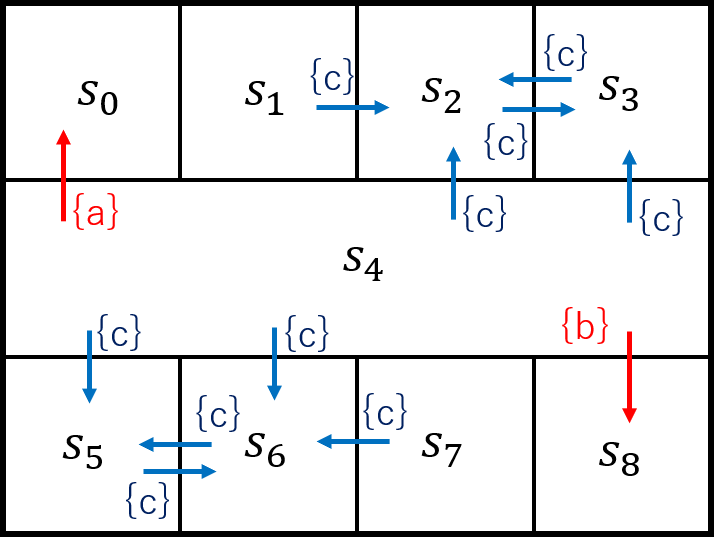
\includegraphics[bb=0 0 377 290,height=4cm,width=6cm]{MDP_corridor.png}
%    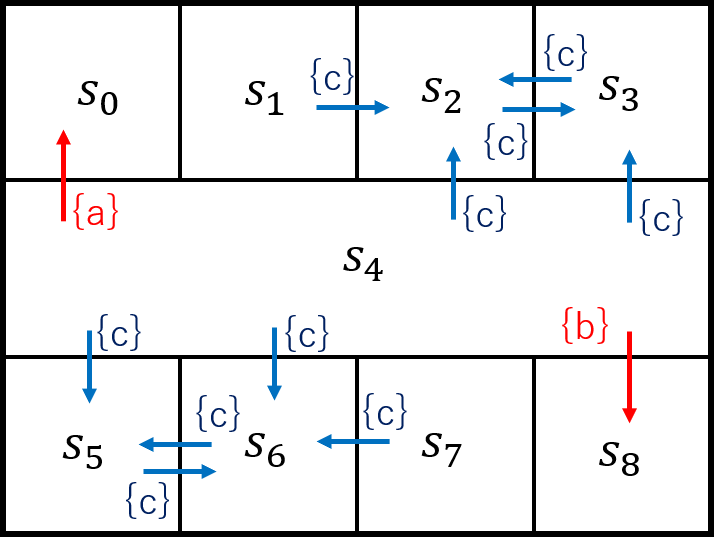
\includegraphics[height=4cm, width=6cm]{MDP_corridor.png}
    \caption{The environment consisting of eight rooms and one corridor. Red arcs are the transitions that we want to occur infinitely often, while blue arcs are the transitions that we never want to occur. $s_7$ is the initial state.}
    \label{Grid1}
\end{figure}

\begin{figure}[htbp]
   \centering
   \vspace{2mm}
%   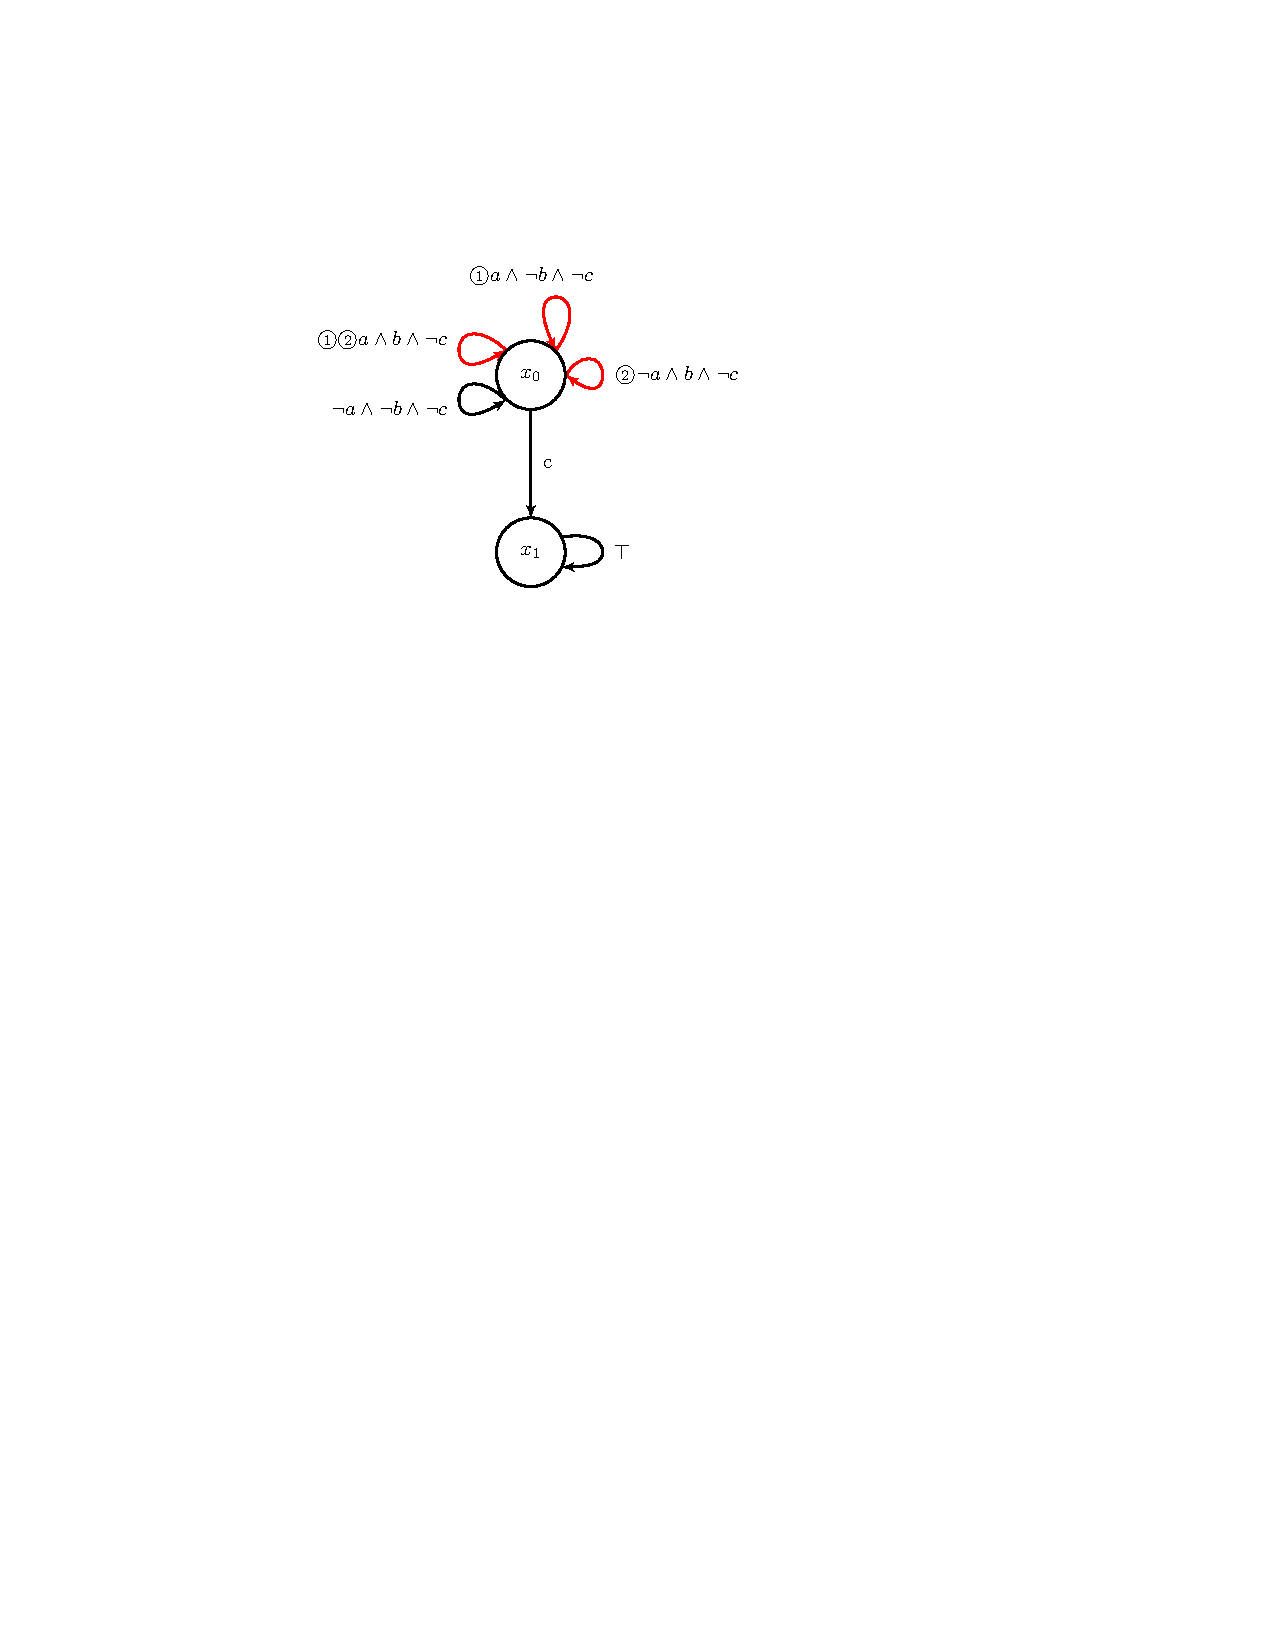
\includegraphics[bb=140 498 368 682,width=5cm]{automaton1.pdf}
   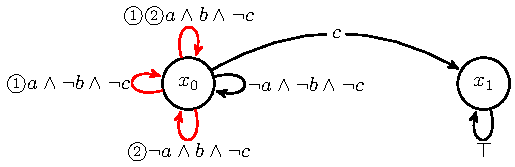
\includegraphics[bb=0 0 247 80,scale=0.85]{ldgba_original.pdf}
   \caption{The tLDBA recognizing the LTL formula $\text{{\bf GF}}a \wedge \text{{\bf GF}}b \wedge \text{{\bf G}}\neg c$, where the initial state is $x_0$. Red arcs are accepting transitions that are numbered in accordance with the accepting sets they belong to, e.g., \textcircled{\scriptsize 1}$a \land \neg b \land \neg c$ means the transition labeled by it belongs to the accepting set $F_1$.}
   \label{automaton}
\end{figure}

\begin{figure}[htbp]
   \centering
%   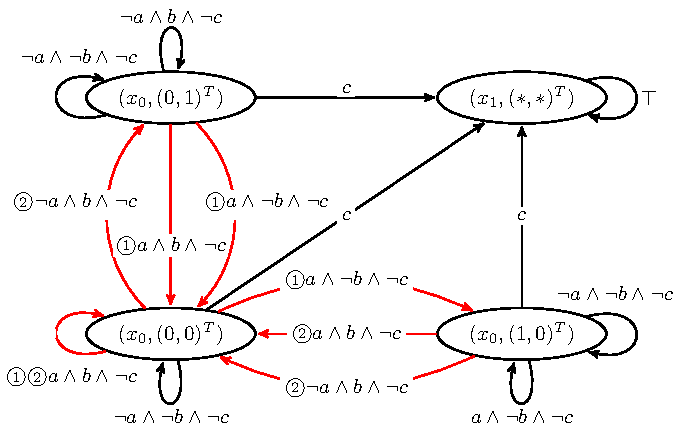
\includegraphics[bb=0 0 374 207,height=4cm, width=7cm]{ldgba.pdf}
   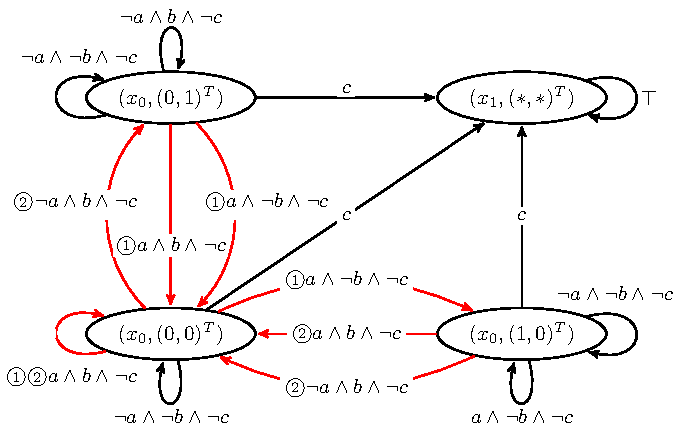
\includegraphics[bb=0 0 374 207,scale=0.75]{ldgba.pdf}
   \caption{The augmented automaton for the tLDBA in Fig.~\ref{automaton} recognizing the LTL formula $\text{{\bf GF}}a \wedge \text{{\bf GF}}b \wedge \text{{\bf G}}\neg c$, where the initial state is $(x_0, (0,0)^T )$. Red arcs are accepting transitions that are numbered in accordance with the accepting sets they belong to. All states corresponding to $x_1$ are merged into $(x_1, (*,*)^T )$.}
   \label{automaton_aug}
\end{figure}

In this section, we evaluate our proposed method and compare it with an existing work.
We consider a path planning problem of a robot in an environment consisting of eight rooms and one corridor as shown in Fig.\ \ref{Grid1}. The state $s_7$ is the initial state and the action space is specified with $\mathcal{A}(s) = \{ Right,\ Left,\ Up,\ Down \}$ for any state $s \neq s_4$ and $\mathcal{A}(s_4) = \{ to\_s_0,\ to\_s_1,\ to\_s_2,$ $\ to\_s_3,\ to\_s_5,\ to\_s_6,\ to\_s_7,\ to\_s_8 \}$, where $to\_s_i$ means attempting to go to the state $s_i$ for $i \in \{0,\ 1,\ 2,\ 3,\ 5,\ 6,\ 7,\ 8 \}$. The robot moves in the intended direction with probability 0.9 and it stays in the same state with probability 0.1 if it is in the state $s_4$. In the states other than $s_4$, it moves in the intended direction with probability 0.9 and it moves in the opposite direction to that it intended to go with probability 0.1. If the robot tries to go to outside the environment, it stays in the same state. The labeling function is as follows.
\begin{align*}
      & L((s, a, s^{\prime})) =
      \left\{
      \begin{aligned}
        & \{ c \} &  & \text{if }s^{\prime} = s_i,\ i \in \{ 2,3,5,6 \}, \nonumber \\
        & \{ a \} &  & \text{if }(s,a,s^{\prime})=(s_4,to\_s_0,s_0), \nonumber \\
        & \{ b \} &  & \text{if }(s,a,s^{\prime})=(s_4,to\_s_8, s_8), \nonumber \\
        & \emptyset &  & \text{otherwise}.
      \end{aligned}
      \right.
    \end{align*}

In the example, the robot tries to take two transitions that we want to occur infinitely often, represented by arcs labeled by \{{\it a}\} and \{{\it b}\}, while avoiding unsafe transitions represented by the arcs labeled by \{{\it c}\}. This is formally specified by the following LTL formula.
\begin{align*}
  \varphi = \text{{\bf GF}}a \wedge \text{{\bf GF}}b \wedge \text{{\bf G}}\neg c.
\end{align*}
The above LTL formula requires the robot to keep on entering the two rooms $s_0$ and $s_8$ from the corridor $s_4$ regardless of the order of entries, while avoiding entering the four rooms $s_2$, $s_3$, $s_5$, and $s_6$.

We use Owl \cite{Owl} to obtain the tLDBA corresponding to the LTL formula.
The tLDBA $B_{\varphi} = (X, x_{init},\Sigma,\delta,\mathcal{F})$ and its augmented automaton $\bar{B}_{\varphi} = (\bar{X},\bar{x}_{init},\bar{\Sigma},\bar{\delta},\bar{\mathcal{F}})$ are shown in Figs.\ \ref{automaton} and \ref{automaton_aug}, respectively. Specifically, the acceptance condition ${\mathcal F}$ of the tLDBA is given by ${\mathcal F} = \{ F_1,F_2 \}$, where $F_1=\{ (x_0, \{ a \}, x_0),\ (x_0, \{ a,b \}, x_0) \}$ and $F_2 = \{ (x_0, \{ b \}, x_0),\ (x_0, \{ a,b \}, x_0) \}$.

We use Q-learning with $\varepsilon$-greedy policy and gradually reduce $\varepsilon$ to 0 to learn an optimal policy asymptotically.
We set the positive reward $r_p = 2$, the epsilon greedy parameter $ \varepsilon = \frac{0.95}{n_t(s^{\otimes})}$, where $n_t(s^{\otimes})$ is the number of visits to state $s^{\otimes}$ within $t$ time steps \cite{Singh1998}, and the discount factor $\gamma = 0.9$. The learning rate $\alpha$ varies in accordance with {\it the Robbins-Monro condition}.

We also evaluate the method by Hasanbeig $et\ al.$\cite{HAK2019} with the same example. They use state-based LDBAs for LTL formulas and construct the product MDP of an MDP and a state-based LDBA to synthesize a policy satisfying the LTL formula. They proposed the accepting frontier function $Acc : X \times 2^X \rightarrow 2^X $ where $X$ is the set of states of the state-based LDBA. Under initializing a set of states $ \mathbb{F} $ with the union of the all accepting sets of the state-based LDBA, the function receives the state $x$ after each transition and the set $\mathbb{F}$. If $x$ is in $\mathbb{F}$, then $Acc$ removes the accepting sets containing $x$ from $\mathbb{F}$. The reward function is based on the varying set $\mathbb{F}$. We conduct the same example with their method using the tLDBA instead.

Figs.\ \ref{result} and \ref{optimal} show the average reward and the optimal policy, respectively, as a result of the learning when using our proposed method and the method in \cite{HAK2019} after 10000 iterations and 1000 episodes. The arithmetic mean of average reward in each episode for 20 learning sessions is displayed per 100 episodes in Fig.\ \ref{result}.

The results suggest that our proposed method can synthesize a policy satisfying $\varphi$ on the MDP, while the method in \cite{HAK2019} cannot. This is because it is impossible that the transitions labeled by $\{ a \}$ and $\{ b \}$ occur from $s_4$ infinitely often by any positional policy with the tLDBA. In detail, the state of the tLDBA is always $x_0$ while the agent does not move to states $s_2$, $s_3$, $s_5$, and $s_6$. Thus, the state of the product MDP is always $(s_4, x_0)$ while the agent stays in $s_4$. Therefore, the method in \cite{HAK2019} may not synthesize policies satisfying LTL specifications depending on the setting of MDPs or LTL specifications.

\begin{figure}[tbp]
 \centering
 \begin{tabular}{c}
  \begin{minipage}{0.5\hsize}
     \centering
%     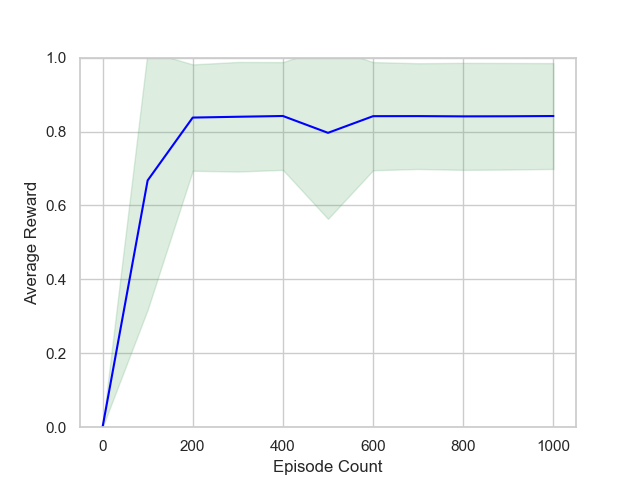
\includegraphics[width=4.5cm]{ep_1000_it_10000_MDP3_gamma_095_re2_ini22_nts_c095_20times.png}
     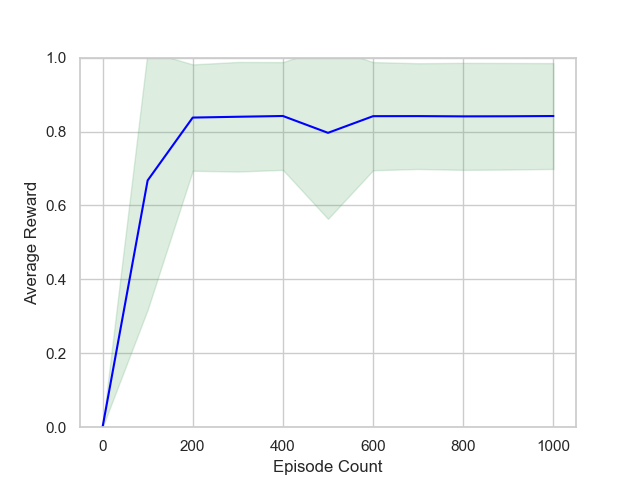
\includegraphics[bb=0 0 461 346, height = 5cm, width=7cm]{ep_1000_it_10000_MDP3_gamma_095_re2_ini22_nts_c095_20times.png}
 \end{minipage}

 \begin{minipage}{0.5\hsize}
   \centering
%   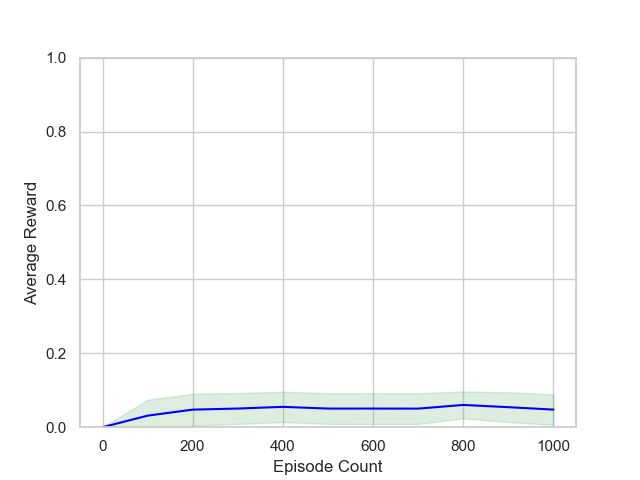
\includegraphics[width=4.5cm]{ep_1000_it_10000_MDP3_gamma_095_nts_c095_abate_20times.png}
   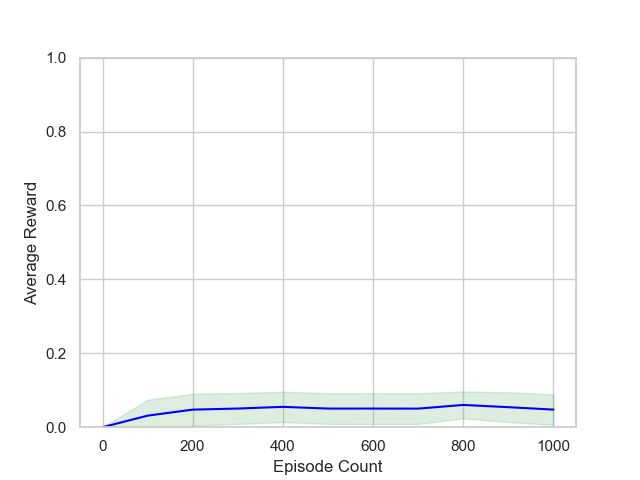
\includegraphics[bb=0 0 461 346, height = 5cm, width=7cm]{ep_1000_it_10000_MDP3_gamma_095_nts_c095_abate_20times.png}
 \end{minipage}
\end{tabular}
 \caption{The arithmetic mean of average reward in each episode for 20 learning sessions obtained from our proposed method (left) and the method by Hasanbeig $et\ al.$\cite{HAK2019} (right). They are plotted per 100 episodes and the green areas represent the range of standard deviations.}
 \label{result}
\end{figure}

\begin{figure}[tbp]
	\centering
	\begin{tabular}{c}

		\begin{minipage}{0.499\hsize}
			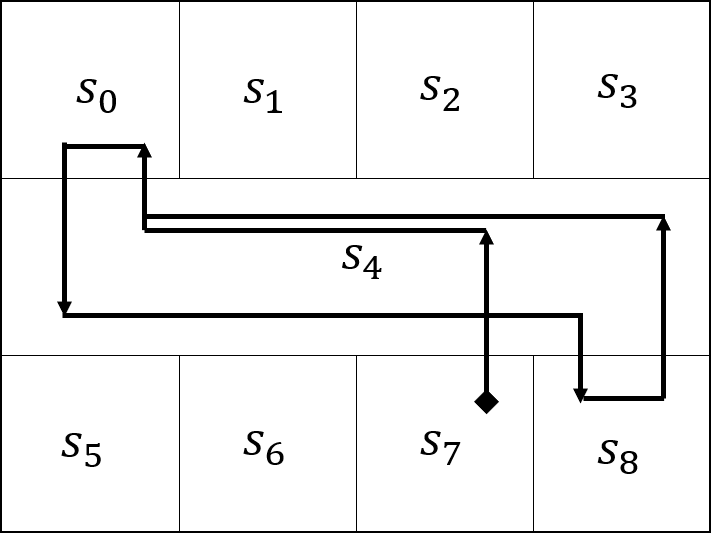
\includegraphics[bb=0 0 341 256, height = 3.7cm, width=5.5cm]{proposed_policy.png}
		\end{minipage}

		\begin{minipage}{0.499\hsize}
			\centering
			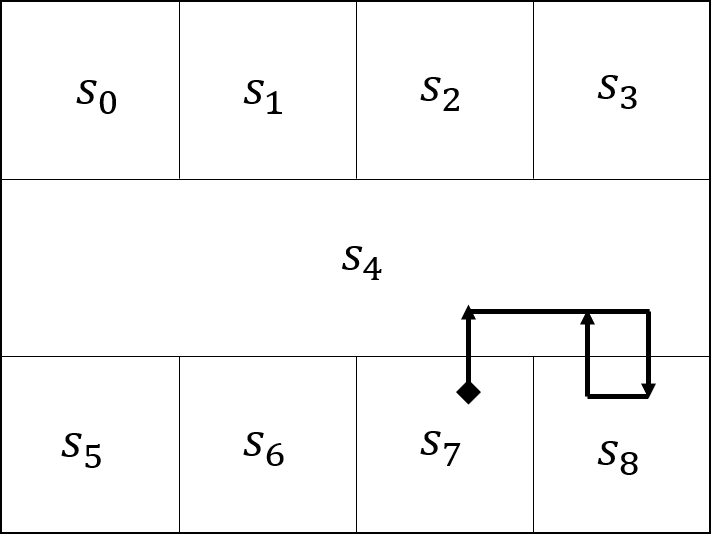
\includegraphics[bb=0 0 341 257, height = 3.7cm, width=5.5cm]{Abate_policy.png}
		\end{minipage}
	\end{tabular}

	\caption{The optimal policy obtained from our proposed method (left) and the method by Hasanbeig $et\ al.$\cite{HAK2019} (right).}
	\label{optimal}
\end{figure}

%%%%%%%%%%%% 4th Chapter %%%%%%%%%%%%%%%%%%%%%%%%%%%%%%%%%%%%%%%%%%%%%%%%%%%
\chapter{4th Chapter}


\begin{definition}
  The two reward functions $\mathcal{R}_1 : S^{\otimes} \times 2^{E^{\otimes}} \rightarrow \mathbb{R}$ and $\mathcal{R}_2 : S^{\otimes} \times E^{\otimes} \times S^{\otimes} \rightarrow \mathbb{R}$ are defined as follows.
  \begin{align}
    \mathcal{R}_1 (s^{\otimes}, \pi) = r_{n1} (|E|-|\pi|),
  \end{align}
  where $|E|$ means number of elements in the set $E$ and $r_{n1}$ is a negative value.
  \begin{align}
    \mathcal{R}_2(s^{\otimes}, e, s^{\otimes \prime}) =
    \left\{
    \begin{aligned}
      &r_p \  \text{if}\ \exists i \in \! \{ 1, \ldots ,n \},\ (s^{\otimes}, e, s^{\otimes \prime}) \in \bar{F}^{\otimes}_i \!,\\
      &r_{n2} \ \text{if}\ \myspdq \in SinkSet,\\
      &0   \ \ \text{otherwise},
    \end{aligned}
    \right.
  \end{align}
\end{definition}
\section{Learning Algorithm}
We make the supervisor learn how to give the control patterns to satisfy an LTL specification while keeping costs associated with prohibited events low. We use Q-learning to estimate the function $T^{\ast}$. We then use Bayesian inference to robustly estimate the probability $P_E$. For the inference, we model $P_E$ as Categorical distribution as $p^k_{s,\pi,e}$, where $p^k_{s,\pi,e}$ represents the estimated probability of $P_E(e|s,\pi)$ at the time step $k$ and the prior distribution $\phi^k_{s,\pi}$ for the parameter of $p^k_{s,\pi,e}$ is defined as Dirichlet.
%Let $\mathcal{P}_{s,\pi}$ be the collection of the estimated probabilities of $P_E(e|s,\pi)$ with respect to all $e \in \pi$.

To reflect the events prohibition by the supervisor on the estimated probability of the occurrence of allowed events, we introduce the function $RestProb : (0,1)^{|E|} \times 2^E \rightarrow [0,1]^{|E|}$ defined as

\begin{align}
  RestProb(\phi_{s,\pi},\pi)_i =
  \left\{
  \begin{aligned}
    & \frac{\phi^i_{s,\pi}}{\sum_{e_j \in \pi} \phi^j_{s,\pi}} \  &\text{if}\ e_i \in \pi,\\
    &0   \ &\text{otherwise},
  \end{aligned}
  \right.
\end{align}
where $\phi^i_{s,\pi}$ is the $i$-th element of $\phi_{s,\pi}$ and $RestProb(\phi_{s,\pi},\pi)_i$ is the $i$-th element of $RestProb(\phi_{s,\pi},\pi)$.

Let $p^k_{s,\pi}$ denote the probability vector at the time step $k$ as $p^k_{s,\pi} = (p^k_{s,\pi,e_1}, \ldots, p^k_{s,\pi,e_{|E|}})$. Let $n^k_{s,\pi,e}$ be the number of the occurrence of the event $e \in E$ up to the time step $k$ under the state $s \in S$ and the control pattern $\pi \in \mathcal{E}(s)$, let $n^k_{s,\pi}$ denote $(n^k_{s,\pi,e_1}, \ldots, n^k_{s,\pi,e_{|E|}})$, and let $\bar{p}^k_{s,\pi}$ denote the expected value of $p^k_{s,\pi}$. The procedure of the inference is shown in Algorithm 1.

\begin{algorithm}
 \caption{$P_E$ inference.}
 \begin{algorithmic}[1]
 \renewcommand{\algorithmicrequire}{\textbf{Input:}}
 \renewcommand{\algorithmicensure}{\textbf{Output:}}
 \REQUIRE the event occurrence count $n^k_{s,\pi}$, a threshold $\xi^k_{s,\pi}$ for $p^k_{s,\pi}$
 \ENSURE  the posterior distribution $p^k_{s,\pi}$
  \REPEAT
  \STATE $\phi^k_{s,\pi} \sim Dir(\cdot|n^k_{s,\pi})$
  \STATE $p^k_{s,\pi} = RestProb(\phi^k_{s,\pi},\pi)$
  \UNTIL $||p^k_{s,\pi} - \bar{p}^k_{s,\pi}||_1 < \xi^k_{s,\pi}$
 \end{algorithmic}
 \label{bayes}
 \end{algorithm}

Under the estimation of $P_E$, we use TD-learning to estimate $Q^{\ast}$ with the TD-error defined as $\mathcal{R}_1(s^{\otimes},\pi) + \sum_{e \in \pi} p_{s^{\otimes},\pi,e} T(s^{\otimes},e) - Q(s^{\otimes},\pi)$.

We show the all procedure of learning algorithm in Algorithm \ref{alg1}.

\begin{algorithm}
 \caption{RL-based synthesis of a supervisor satisfying a given LTL specification.}
 \begin{algorithmic}[1]
 \renewcommand{\algorithmicrequire}{\textbf{Input:}}
 \renewcommand{\algorithmicensure}{\textbf{Output:}}
 \REQUIRE LTL formula $\varphi$, DES $M$
 \ENSURE  optimal supervisor $SV^{\ast}$ on the product DES $M^{\otimes}$
  \STATE Convert $\varphi$ into tLDBA $B_{\varphi}$.
  \STATE Augment $B_{\varphi}$ to $\bar{B}_{\varphi}$.
  \STATE Construct the product DES $M^{\otimes}$ of $M$ and $\bar{B}_{\varphi}$.
  \STATE Initialize $T:S^{\otimes} \times E^{\otimes} \rightarrow \mathbb{R}$.
  \STATE Initialize $Q:S^{\otimes} \times 2^{E^{\otimes}} \rightarrow \mathbb{R}$.
  \STATE Initialize $n:S^{\otimes} \times 2^{E^{\otimes}} \times E^{\otimes} \rightarrow \mathbb{R}$.
  \STATE Initialize episode length $L$.
  \WHILE {$Q$ is not converged}
  \STATE $s^{\otimes} \leftarrow (s_{init},(x_{init},\bm{0}))$.
  \STATE $t \leftarrow 0$
  \WHILE {$t <L$ and $\myspq \notin SinkSet$ }
  \STATE Choose the control pattern $\pi \in \mathcal{E}(s^{\otimes})$ by the supervisor $SV$.
  \STATE Observe the occurrence of the event $e \in E$.
  \STATE Observe the next state $s^{\otimes \prime}$.
  \STATE $T(s^{\otimes},e) \leftarrow (1-\alpha)T(s^{\otimes},e) + \alpha \{ \mathcal{R}_2(s^{\otimes},e,s^{\otimes \prime}) + \gamma \max_{\pi^{\prime} \in 2^{\mathcal{E}(s^{\otimes \prime})}}Q(s^{\otimes \prime},\pi^{\prime}) \}$
  \STATE $n(s^{\otimes}, \pi, e) \leftarrow n(s^{\otimes}, \pi, e) + 1$
  \STATE Obtain $p_{s^{\otimes},\pi}$ by the $P_E$ inference.
  \STATE $Q(s^{\otimes},\pi) = (1-\beta)Q(s^{\otimes},\pi) + \beta \{\mathcal{R}_1(s^{\otimes},\pi) + \sum_{e \in \pi} p_{s^{\otimes},\pi,e} T(s^{\otimes},e)$\}
  \STATE $s^{\otimes} \leftarrow s^{\otimes \prime}$
  \STATE $t \leftarrow t + 1$
  \ENDWHILE
  \ENDWHILE
 \end{algorithmic}
 \label{alg1}
 \end{algorithm}

\section{Example}
We evaluate the two algorithms by the maze of the cat and the mouse shown in Fig.\ \ref{cat_mouse}. At the beginning, we define the settings for the example. The corresponding DES is as follows. The state set is $S = \{ (s^{cat}, s^{mouse}) ; s^{cat},s^{mouse} \in \{ s_0,s_1,s_2,s_3 \} \}$. The set of events (to open the corresponding door) is $E = \{ m_0, m_1, m_2, m_3, c_0, c_1, c_2, c_3 \}$, where $E_{c} = \{ m_0, m_1, m_2, m_3, c_0, c_1, c_2 \}$ and $E_{uc} = \{ c_3 \}$ and $\mathcal{E}(s) = E$ for any $s \in S$. The initial state is $s_{init} = (s_0, s_2)$. If the door of the room with the cat (resp., mouse) opens, the cat (resp., mouse) moves, with probability 0.95, to the room next to the room with it where the door is open or stays in the same room with probability 0.05. Otherwise, the cat (resp., mouse) stays in the same room with probability 1. The labeling function is

\begin{align}
   L((s, a, s^{\prime})) =
    \left\{
    \begin{aligned}
      & \{ a \} &  & \text{if }s_c^{\prime} = s_1, \nonumber \\
      & \{ b \} &  & \text{if }s_m^{\prime} = s_1, \nonumber \\
      & \{ c \} &  & \text{if }s_c^{\prime} = s_m^{\prime}, \nonumber \\
      & \emptyset &  & \text{otherwise},
    \end{aligned}
    \right.
\end{align}
where $s_c^{\prime}$ and $s_m^{\prime}$ is the next room where the cat and the mouse is, respectively, i.e., $s^{\prime} = (s_c^{\prime},s_m^{\prime})$.

In the example, we want the supervisor to learn to give control patterns satisfying that the cat and the mouse take the food in the room 1 ($s_1$) avoiding they come across. This is formally specified by the following LTL formula.
\begin{align*}
  \varphi = \text{{\bf GF}}a \wedge \text{{\bf GF}}b \wedge \text{{\bf G}}\neg c.
\end{align*}
The tLDBA $B_{\varphi} = (X, x_{init},\Sigma,\delta,\mathcal{F})$ corresponding to $\varphi$ is shown in Fig.\ \ref{tldba}. $B_{\varphi}$ has the acceptance condition of two accepting sets.

We use $\varepsilon$-greedy policy and gradually reduce $\varepsilon$ to 0 to learn an optimal supervisor asymptotically.
We set the rewards $r_p = 10$, $r_{n1} = -0.1. -0.5, and -1$, and $r_{n2} = -100$; the epsilon greedy parameter $ \varepsilon = \frac{1}{ \sqrt{episode} }$, where $episode$ is the number of the current episode; and the discount factor $\gamma = 0.99$. $\xi^k_{s^{\otimes},\pi}$ is initially set to 1 and changes to 0.6 during 1/3 to 2/3 of all episodes and to 0.3 after 2/3 of all episodes for any $(s^{\otimes},\pi) \in S^{\otimes} \times 2^{E^{\otimes}}$. The learning rate $\alpha$ and $\beta$ vary in accordance with {\it the Robbins-Monro condition}.

Figs.\ \ref{result1}, \ref{result2}, and \ref{result3} show the estimated optimal state value function at the initial state $V(s^{\otimes}_{init})$ with $r_{n1} = -0.1. -0.5,$ and $-1$, respectively, for each episode when learning 5000 iterations and 15000 episodes by the algorithm \ref{alg1}.
Fig.\ \ref{sim1}, \ref{sim2}, and \ref{sim3} shows the average reward from $\mathcal{R}_2$ and the average cost from $\mathcal{R}_1$ with $r_{n1} = -0.1. -0.5,$ and $-1$, respectively, of 5000 iteration and 1000 episodes by the supervisor obtained from the learning.
\begin{comment}
Fig.\ \ref{result3} shows the the average reward from $\mathcal{R}_2$ and the average cost from $\mathcal{R}_1$ as a result of the learning when using the algorithm \ref{alg2} {\bf by the same example and the same parameters except that the epsilon greedy parameter $\bf{ \varepsilon = \frac{1}{episode} }$. }
\end{comment}
\begin{figure}[htbp]
   \centering
   \vspace{2mm}
%   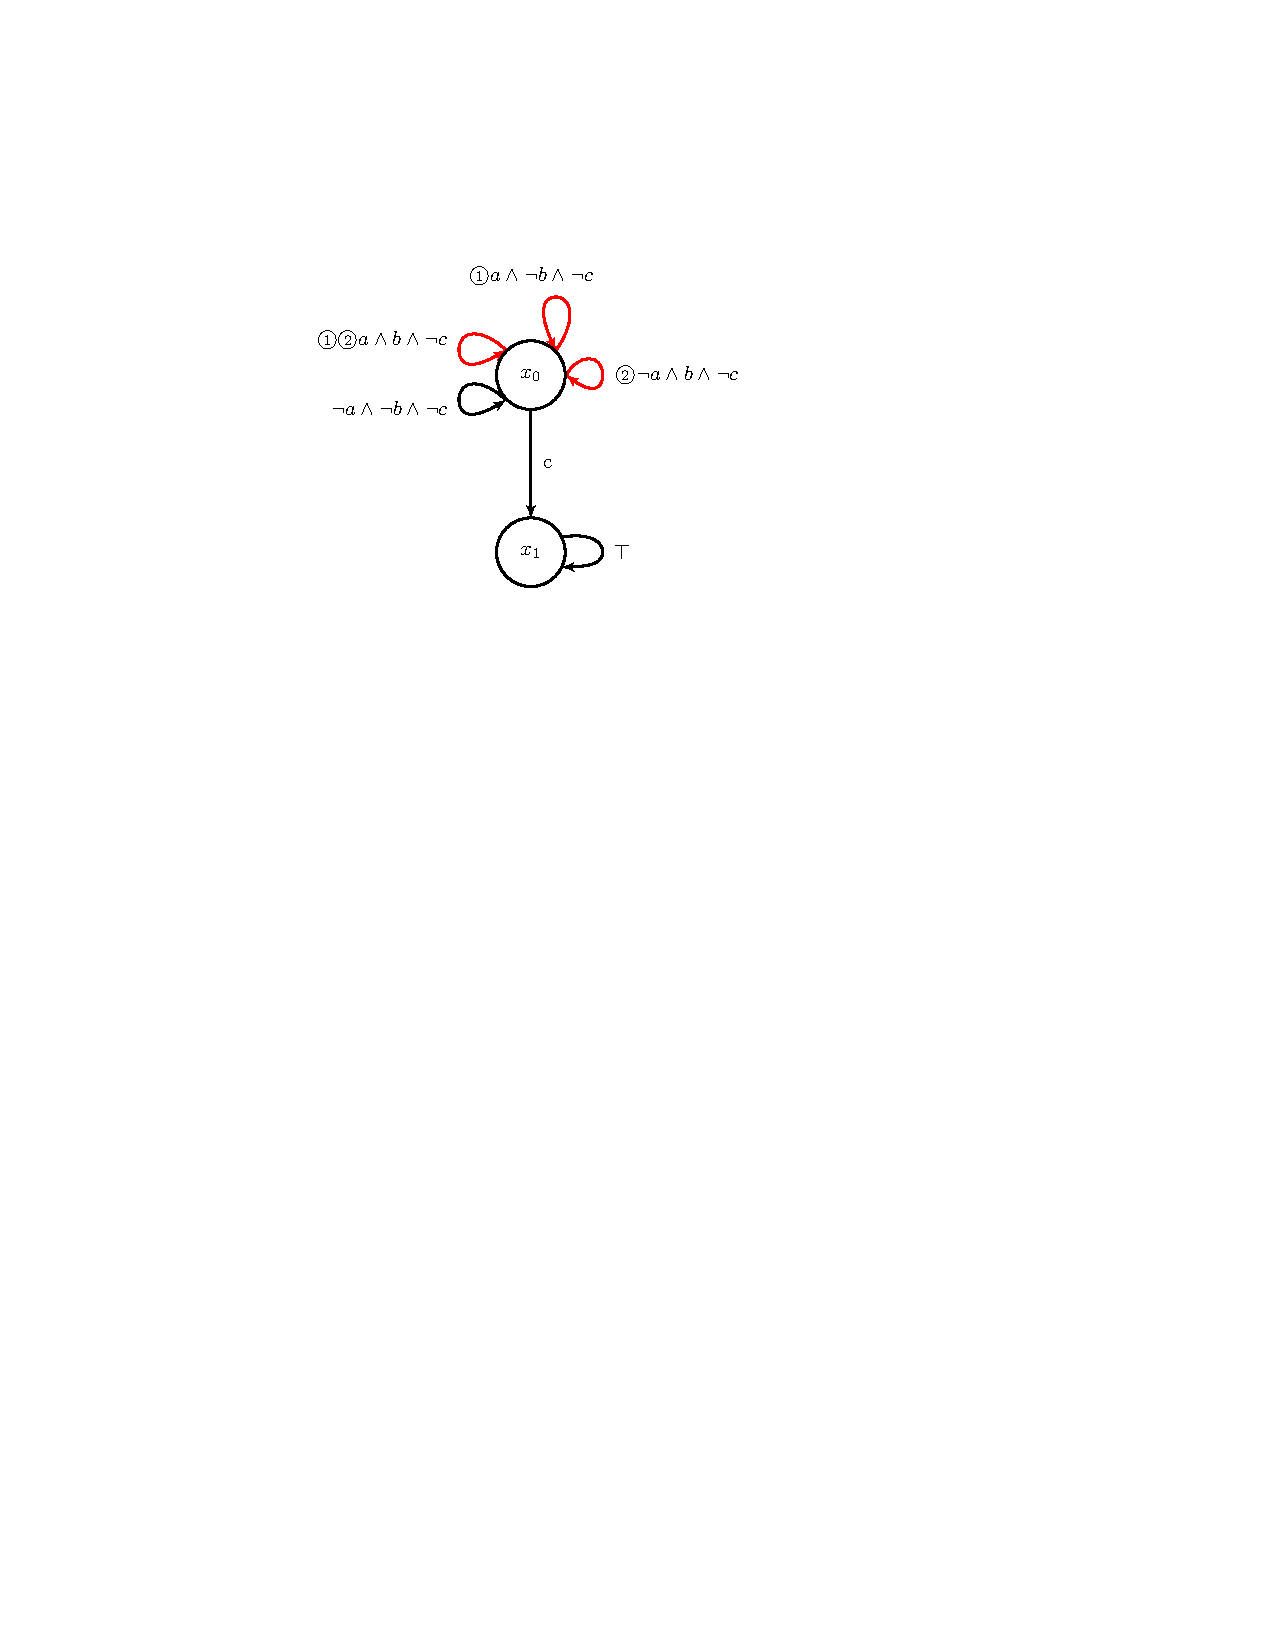
\includegraphics[bb=140 498 368 682,width=5cm]{automaton1.pdf}
   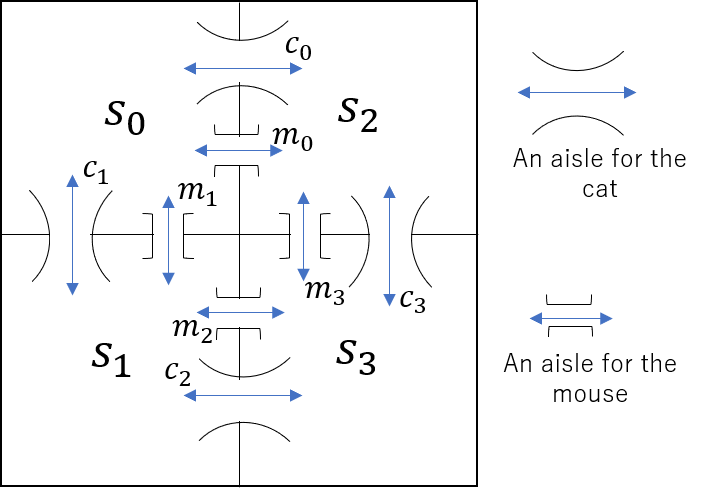
\includegraphics[width=7cm]{cat_mouse.png}
   \caption{The maze of the cat and the mouse. the initial state of the cat and the mouse is $s_0$ and $s_2$, respectively. the food for them is in the room 1 ($s_1$).}
   \label{cat_mouse}
\end{figure}

\begin{figure}[htbp]
   \centering
   \vspace{2mm}
%   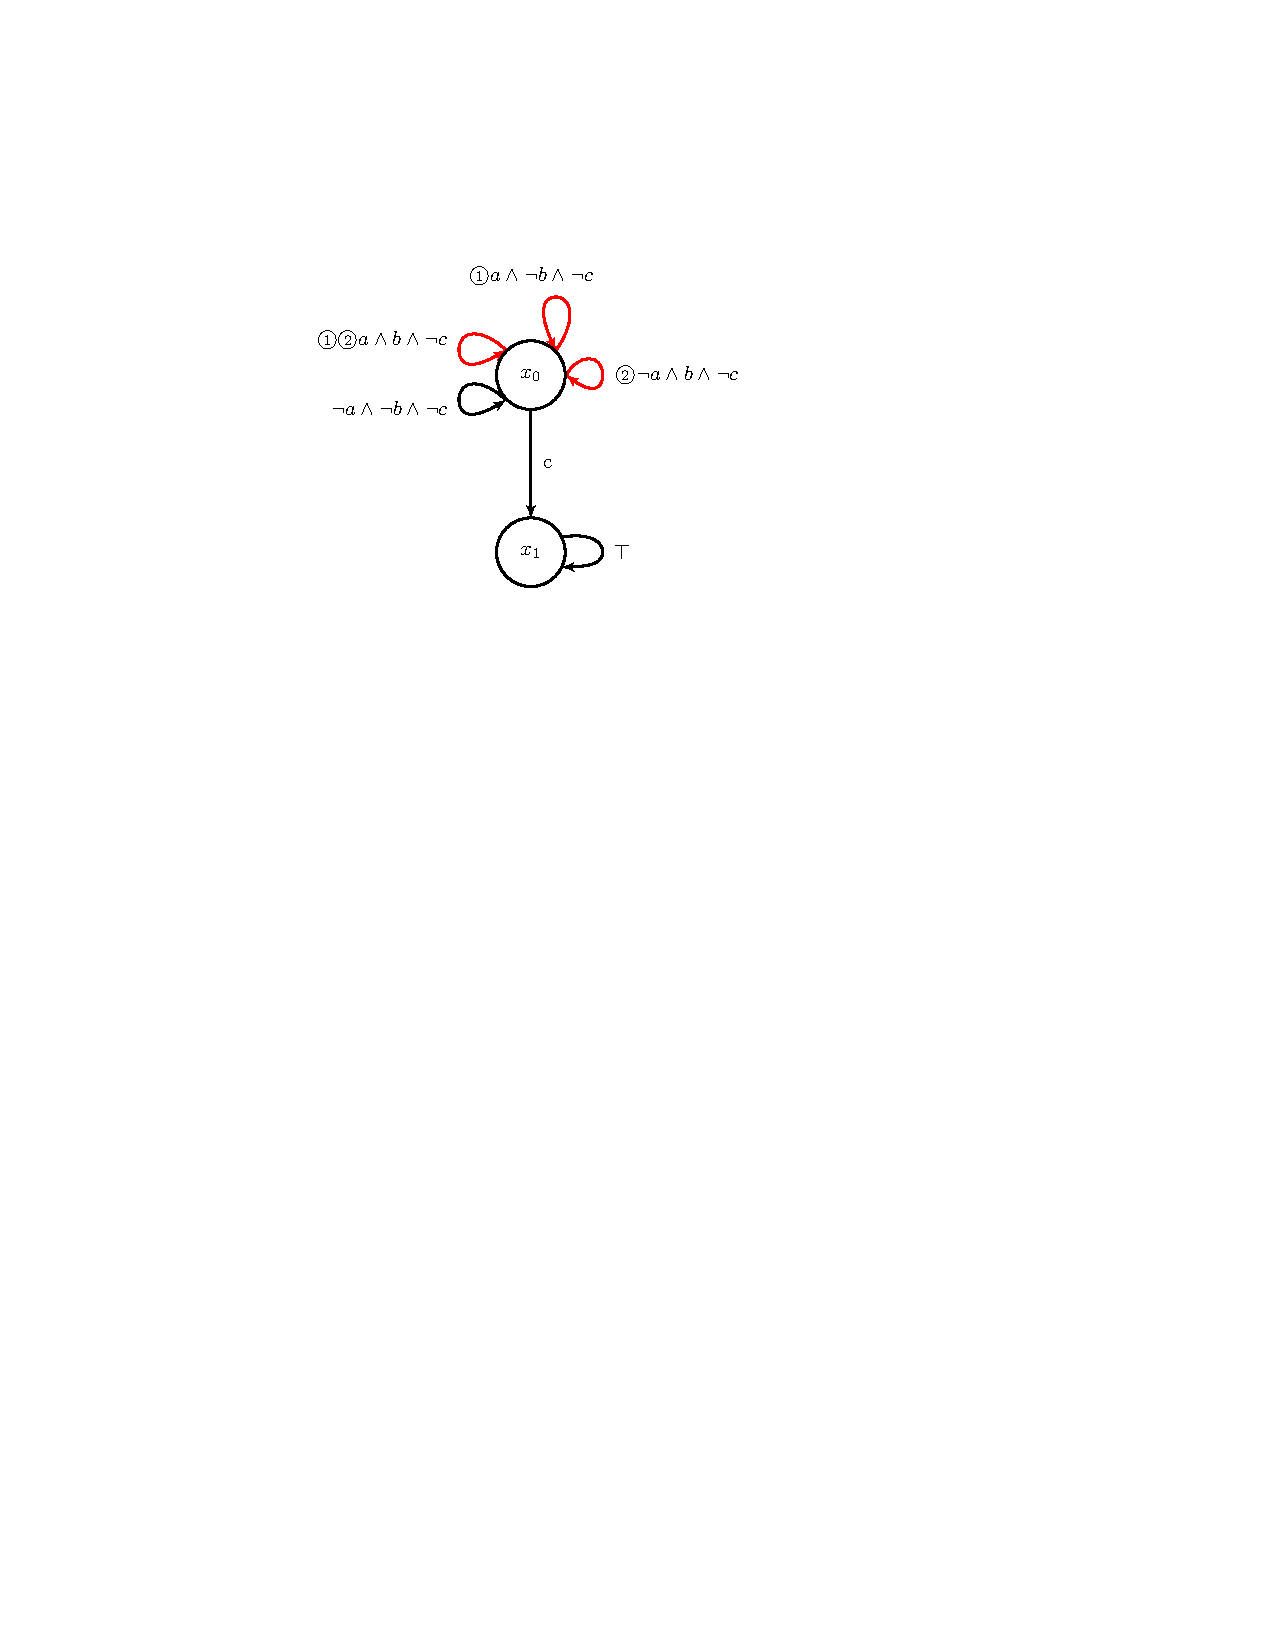
\includegraphics[bb=140 498 368 682,width=5cm]{automaton1.pdf}
   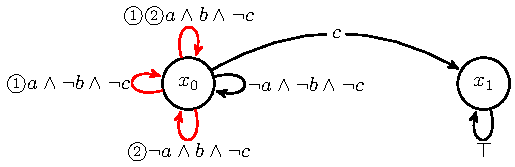
\includegraphics[bb=0 0 247 80,scale=0.85]{ldgba_original.pdf}
   \caption{The tLDBA recognizing the LTL formula $\text{{\bf GF}}a \wedge \text{{\bf GF}}b \wedge \text{{\bf G}}\neg c$, where the initial state is $x_0$. Red arcs are accepting transitions that are numbered in accordance with the accepting sets they belong to, e.g., \textcircled{\scriptsize 1}$a \land \neg b \land \neg c$ means the transition labeled by it belongs to the accepting set $F_1$.}
   \label{tldba}
\end{figure}

\begin{figure}[htbp]
   \centering
   \vspace{2mm}
%   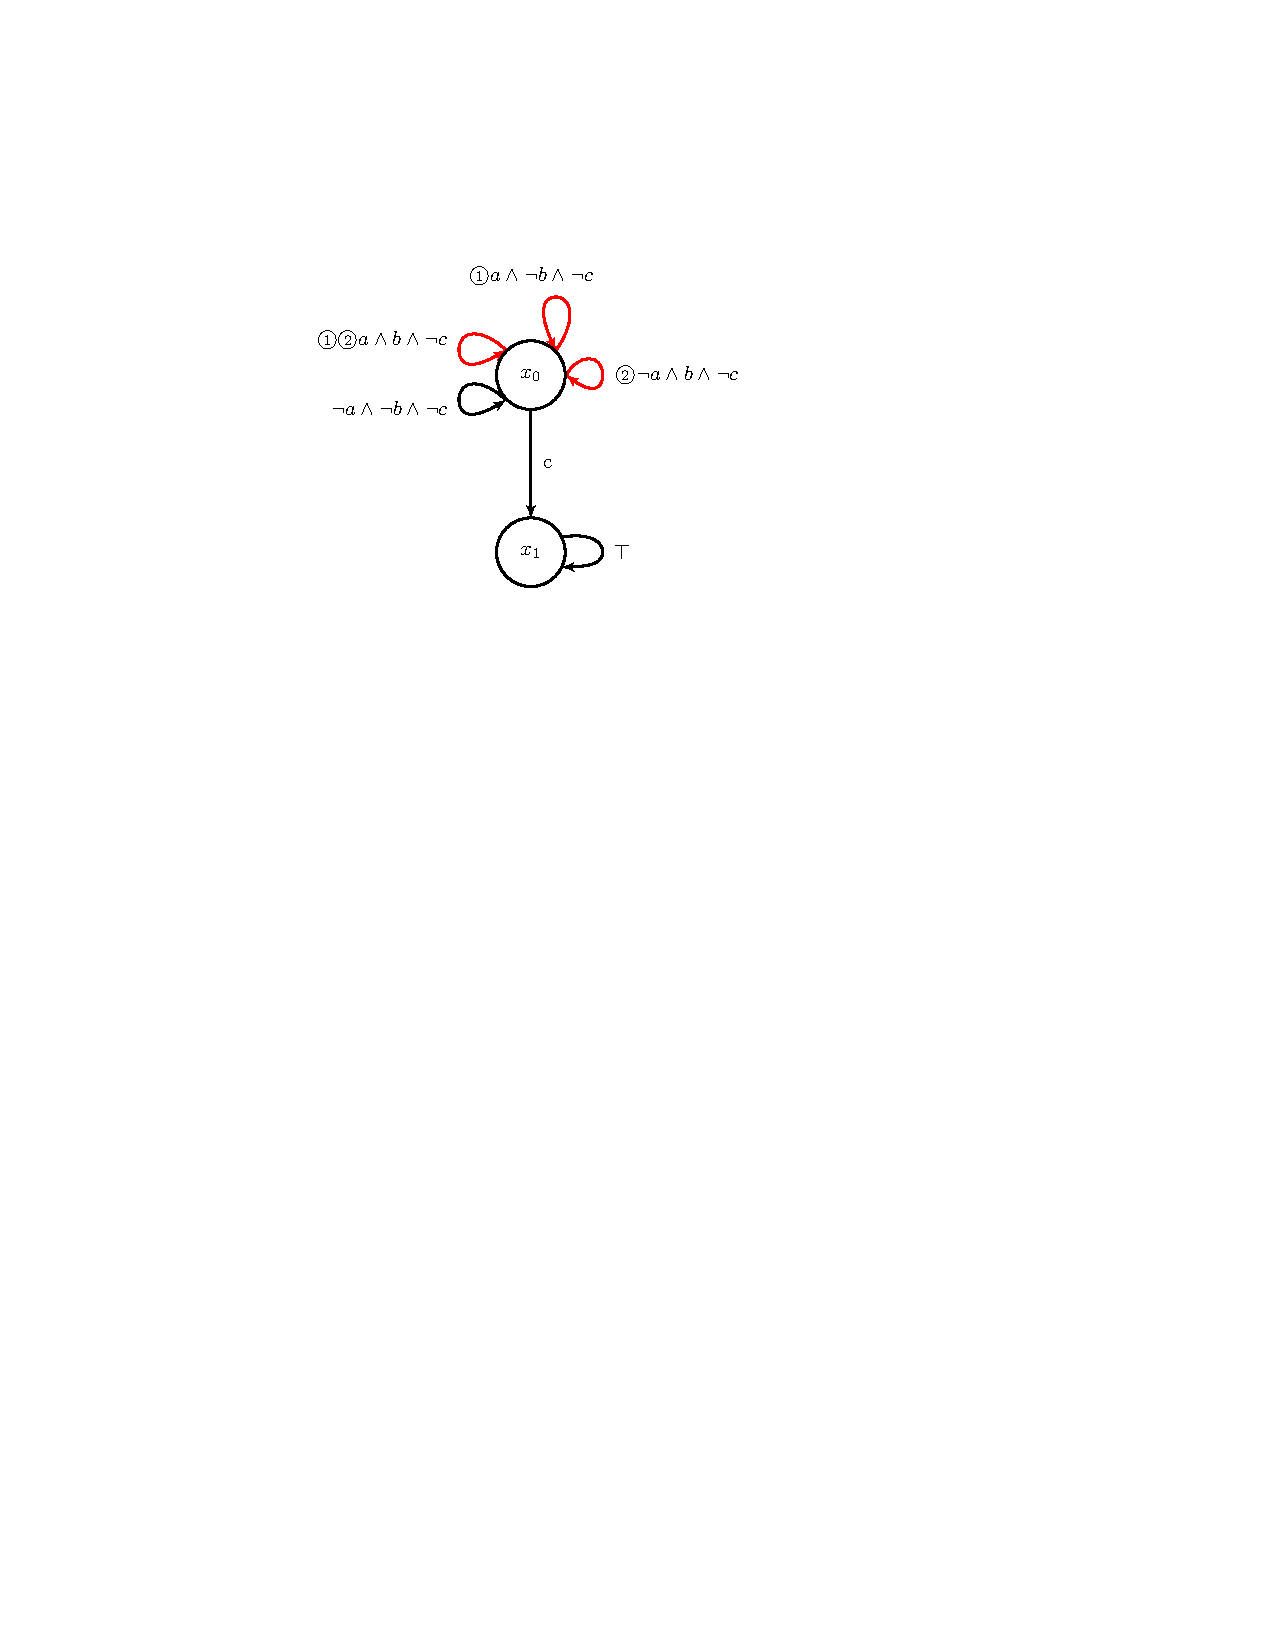
\includegraphics[bb=140 498 368 682,width=5cm]{automaton1.pdf}
   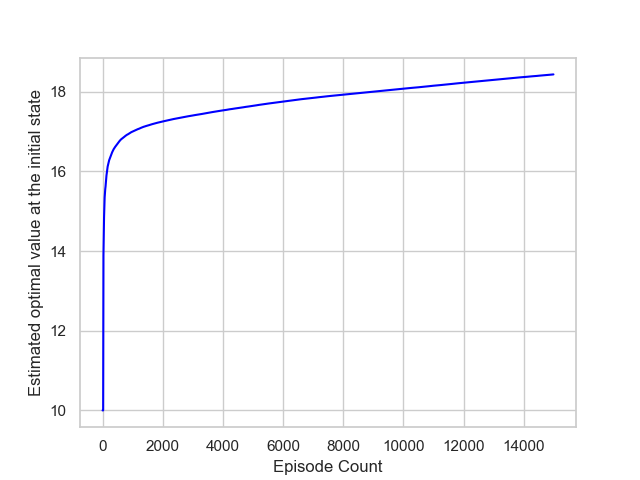
\includegraphics[width = 8cm]{max_Q_value_TD.png}
   \caption{the estimated optimal state value function at the initial state $V(s^{\otimes}_{init})$ with $r_{n1} = -0.1$ when using the algorithm \ref{alg1}.}
   \label{result1}
\end{figure}

\begin{figure}[htbp]
   \centering
   \vspace{2mm}
%   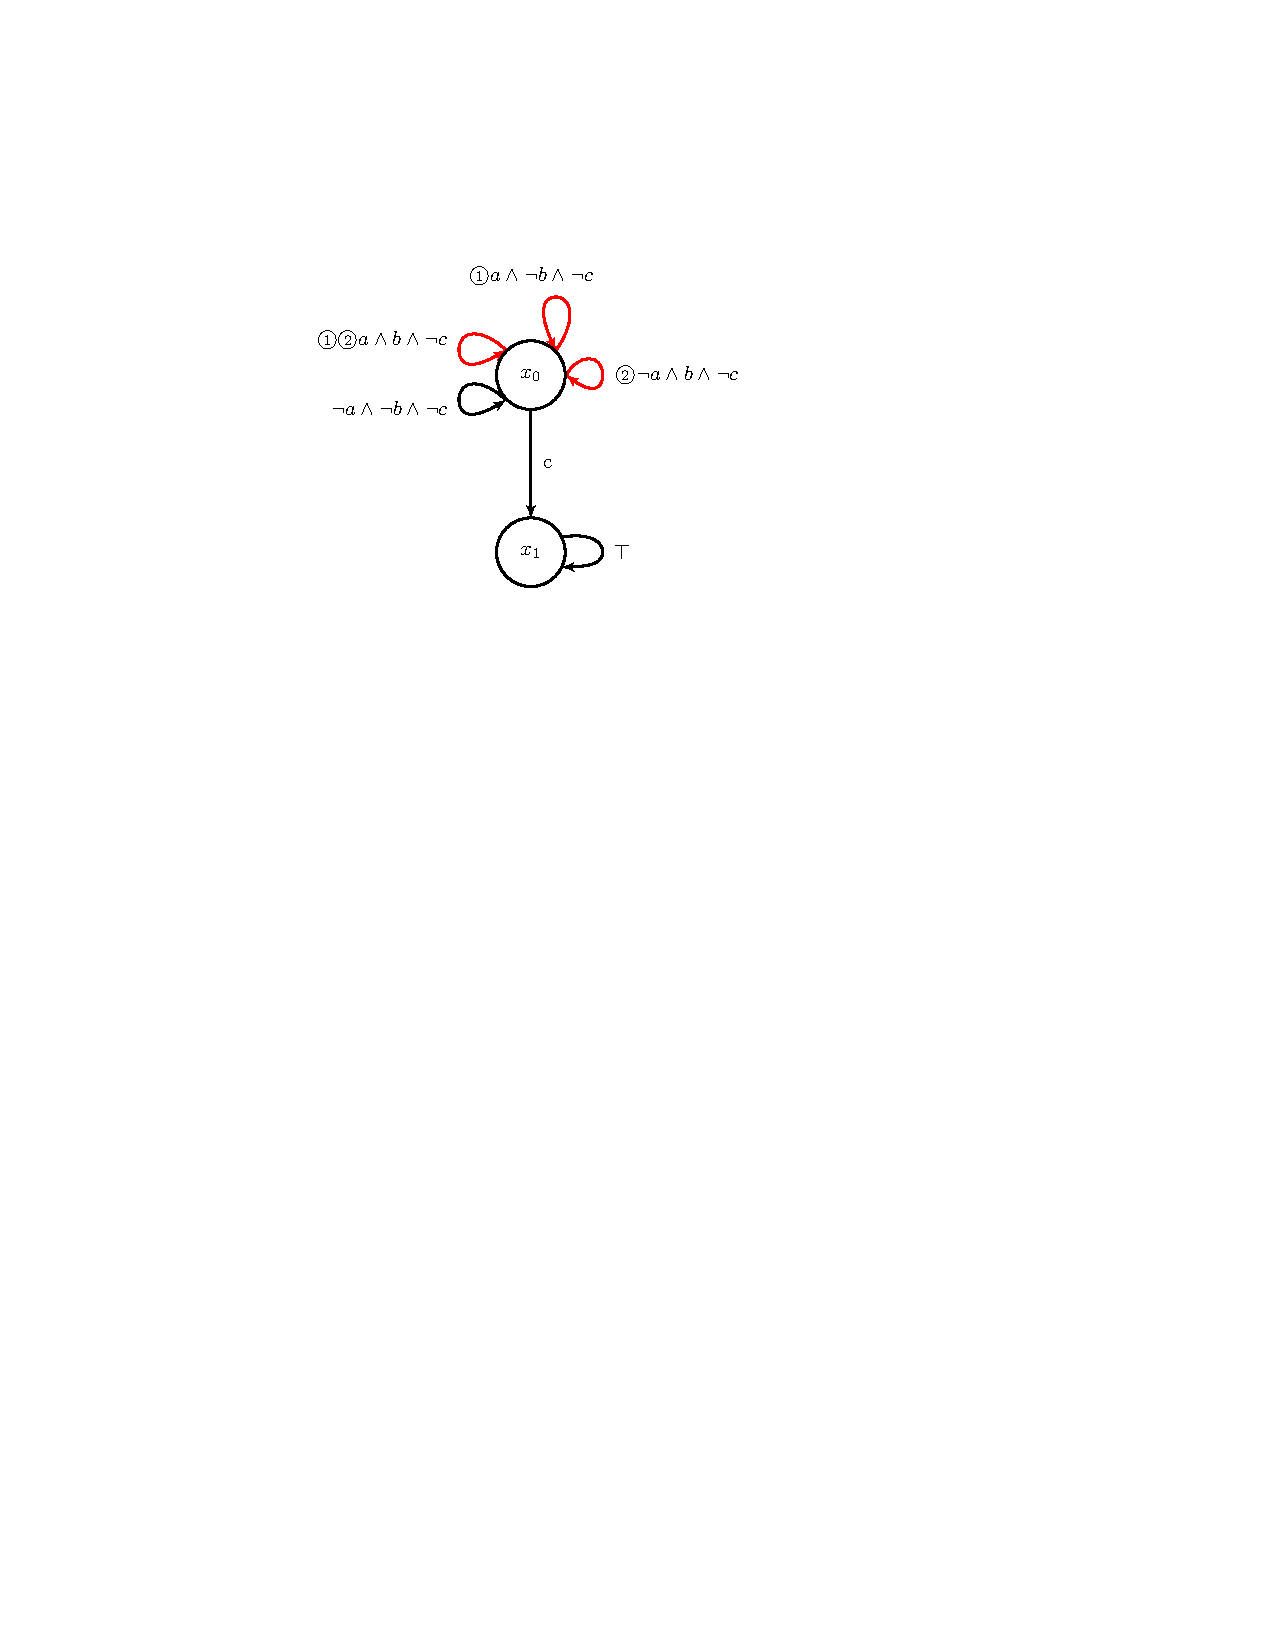
\includegraphics[bb=140 498 368 682,width=5cm]{automaton1.pdf}
   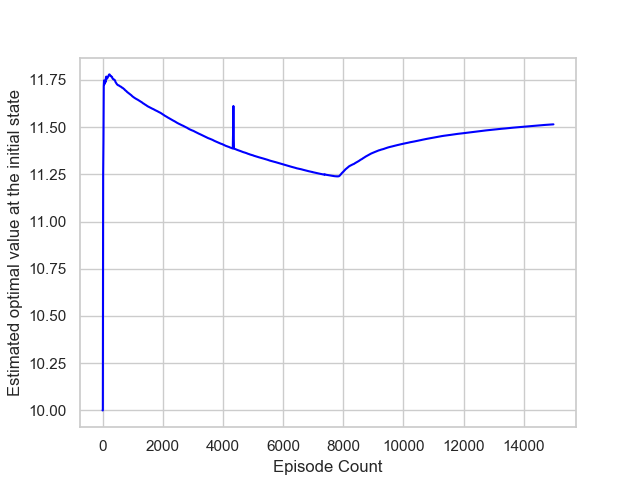
\includegraphics[width = 8cm]{learning_TD_v_15000_5000_rn2_05.png}
   \caption{the estimated optimal state value function at the initial state $V(s^{\otimes}_{init})$ with $r_{n1} = -0.5$ when using the algorithm \ref{alg1}.}
   \label{result1}
\end{figure}

\begin{figure}[htbp]
   \centering
   \vspace{2mm}
%   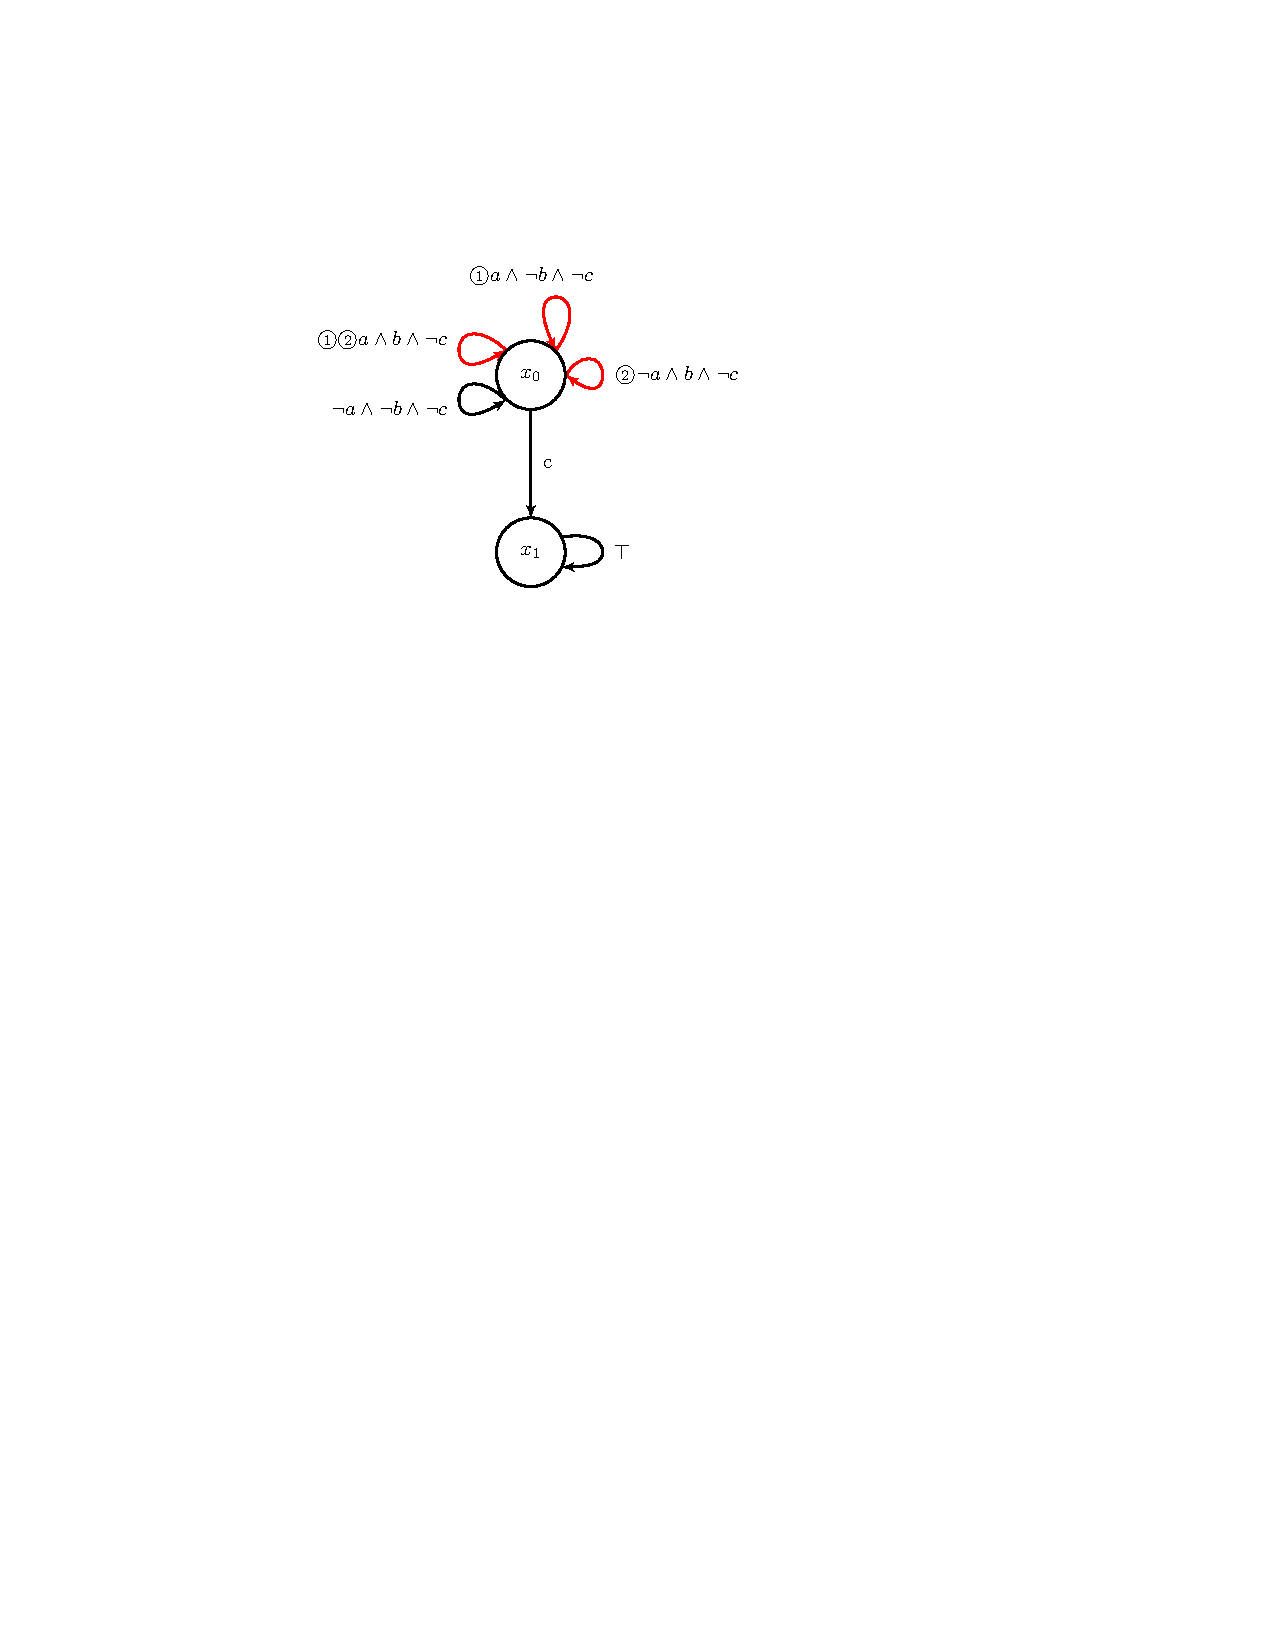
\includegraphics[bb=140 498 368 682,width=5cm]{automaton1.pdf}
   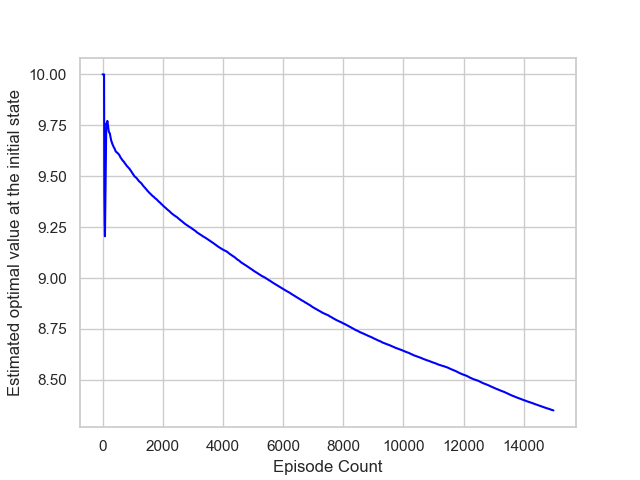
\includegraphics[width = 8cm]{max_Q_value_TD_rn2_1.png}
   \caption{the estimated optimal state value function at the initial state $V(s^{\otimes}_{init})$ with $r_{n1} = -1$ when using the algorithm \ref{alg1}.}
   \label{result1}
\end{figure}

\begin{figure}[htbp]
   \centering
   \vspace{2mm}
%   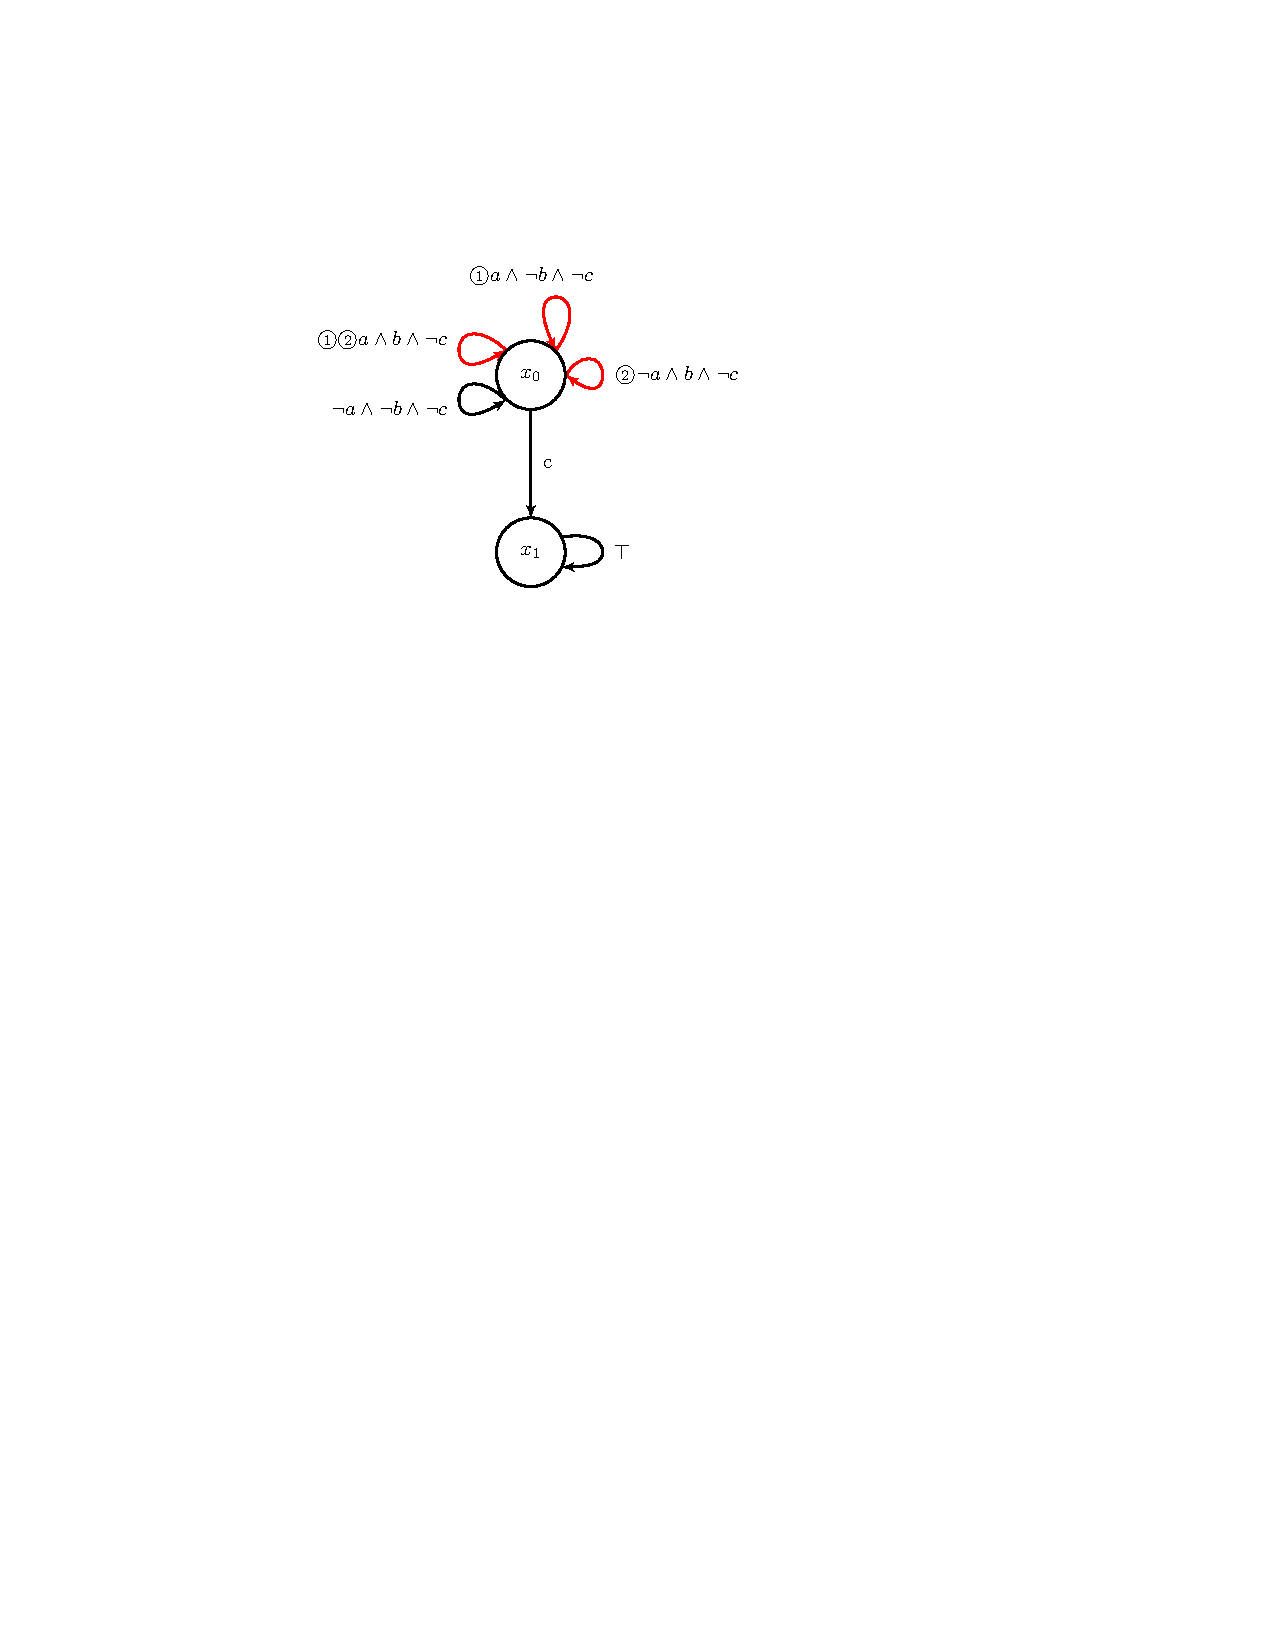
\includegraphics[bb=140 498 368 682,width=5cm]{automaton1.pdf}
   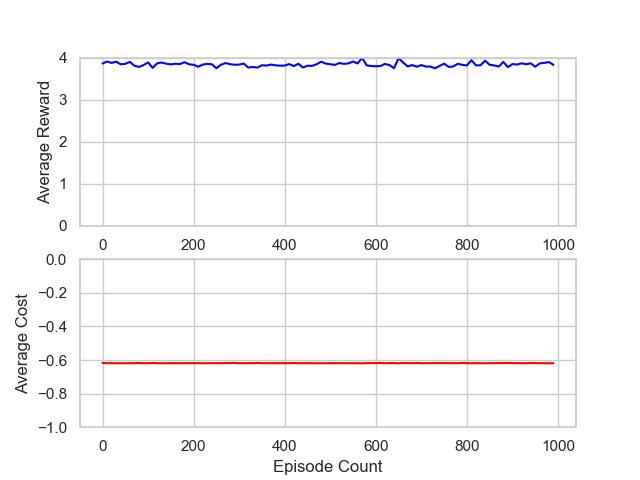
\includegraphics[width = 8cm]{simulate_TD_v_15000_5000.png}
   \caption{The average reward and average cost by the supervisor obtained from the learning with $r_{n1} = -0.1$.}
   \label{sim1}
\end{figure}

\begin{figure}[htbp]
   \centering
   \vspace{2mm}
%   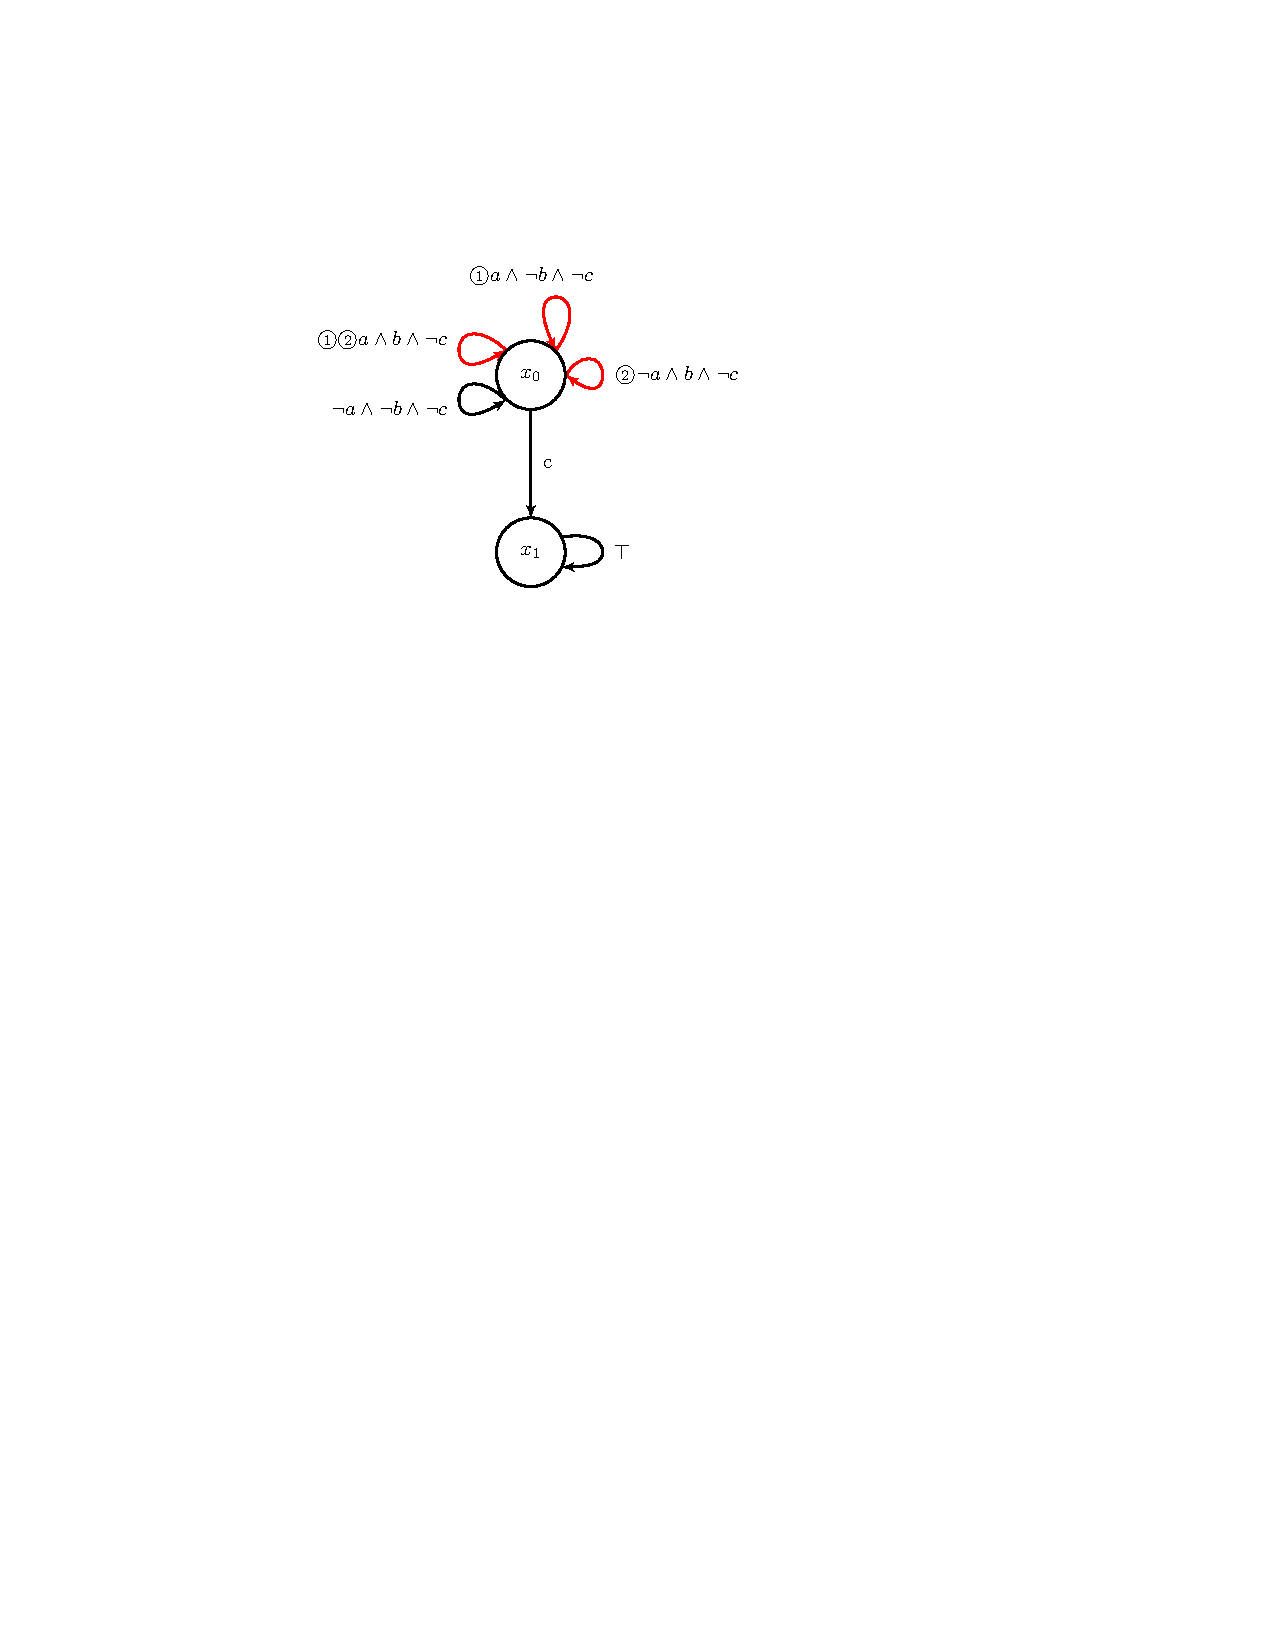
\includegraphics[bb=140 498 368 682,width=5cm]{automaton1.pdf}
   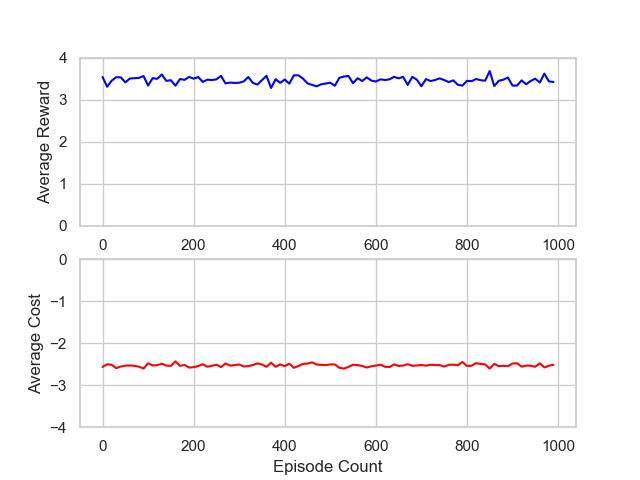
\includegraphics[width = 8cm]{simulate_TD_v_15000_5000_rn2_05.png}
   \caption{The average reward and average cost by the supervisor obtained from the learning with $r_{n1} = -0.5$.}
   \label{sim1}
\end{figure}

\begin{figure}[htbp]
   \centering
   \vspace{2mm}
%   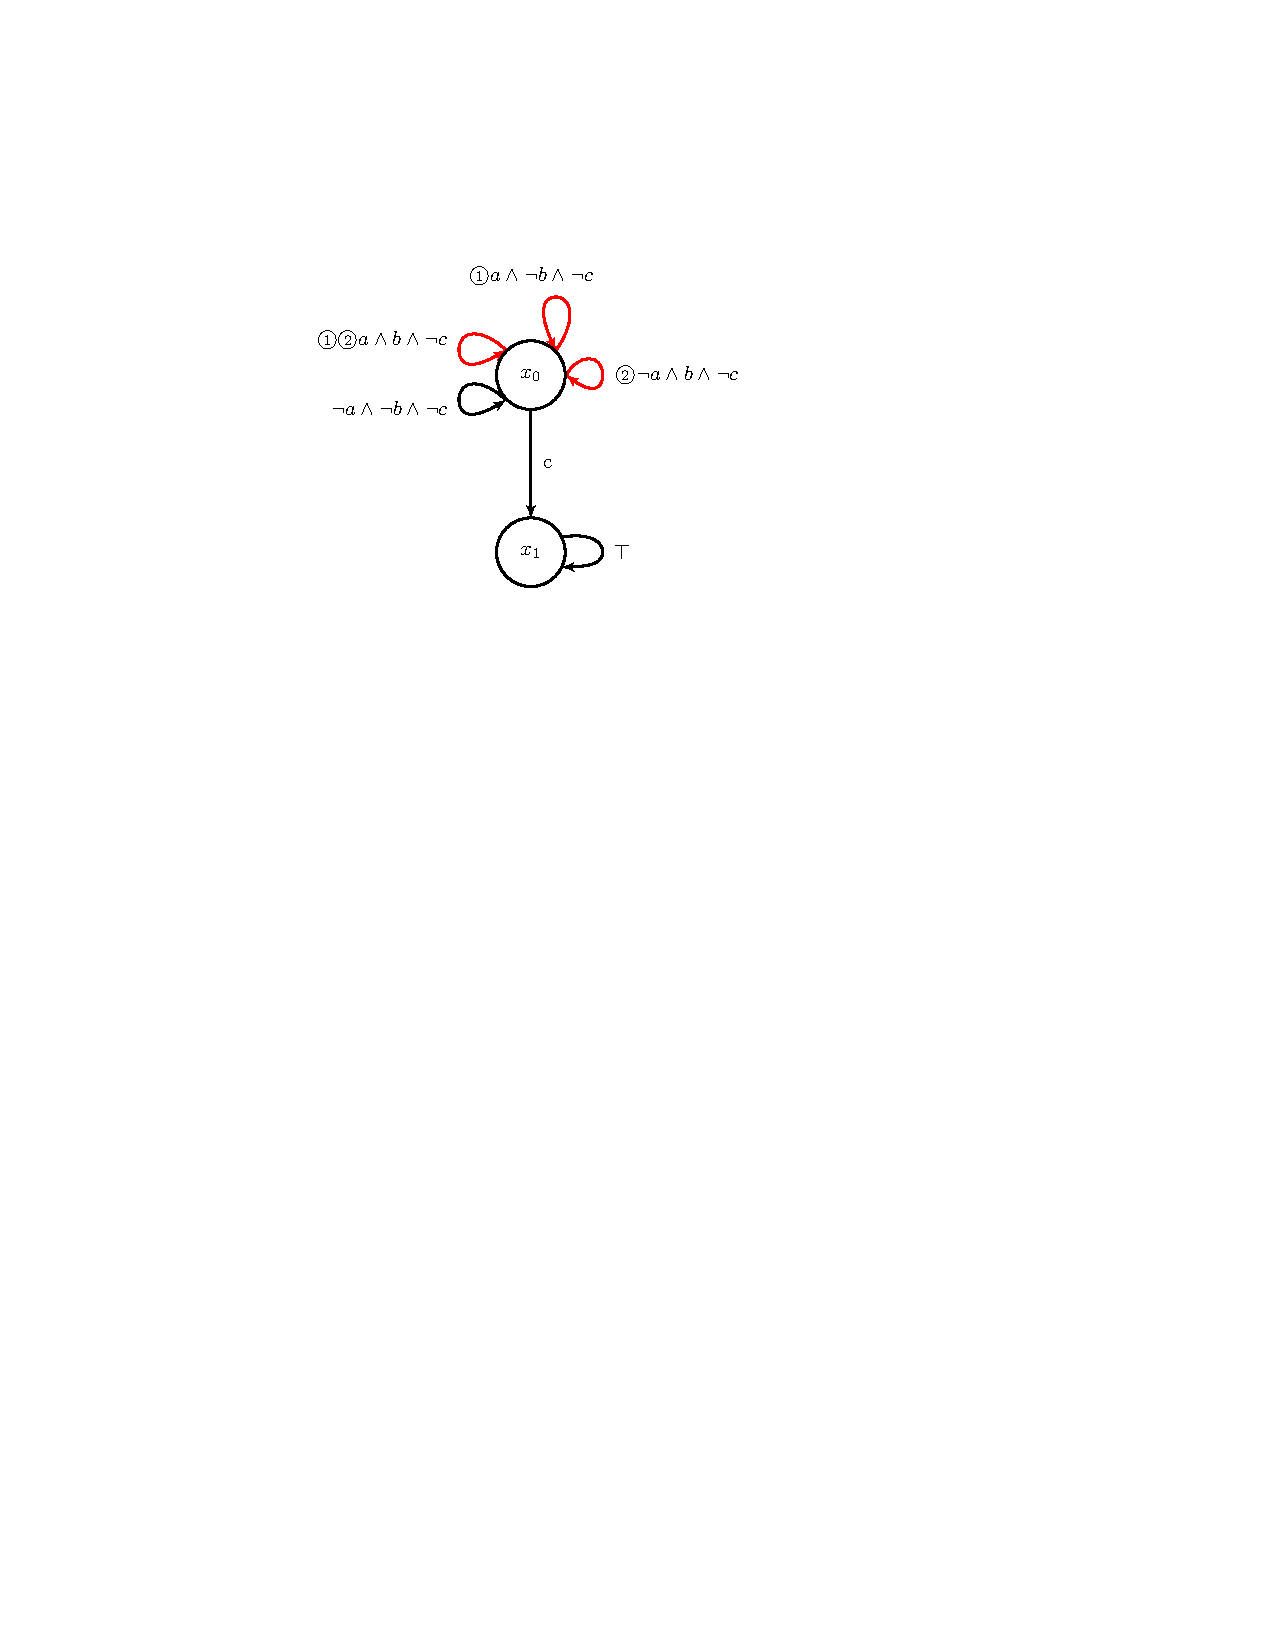
\includegraphics[bb=140 498 368 682,width=5cm]{automaton1.pdf}
   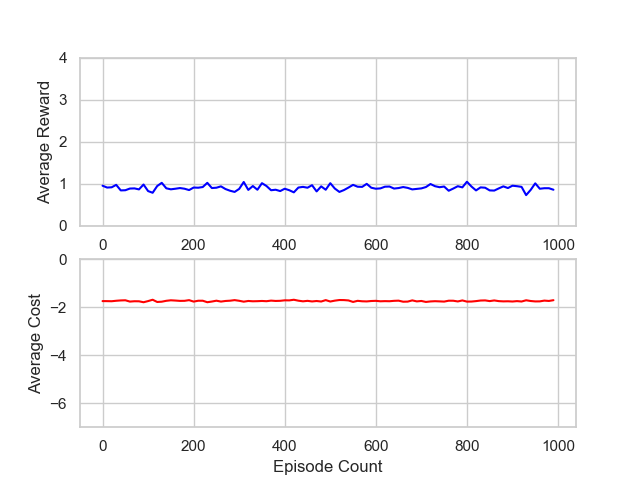
\includegraphics[width = 8cm]{simulate_TD_v_10000_5000_rn2_1.png}
   \caption{The average reward and average cost by the supervisor obtained from the learning with $r_{n1} = -1$.}
   \label{sim1}
\end{figure}

\begin{comment}
\begin{align}
   L((s, a, s^{\prime})) =
    \left\{
    \begin{aligned}
      & \{ a \} &  & \text{if }s_c^{\prime} = s_1, \nonumber \\
      & \{ b \} &  & \text{if }s_m^{\prime} = s_1, \nonumber \\
      & \{ c \} &  & \text{if }s_c^{\prime} = s_2, \nonumber \\
      & \{ d \} &  & \text{if }s_m^{\prime} = s_4, \nonumber \\
      & \{ e \} &  & \text{if }s_c^{\prime} = s_m^{\prime}, \nonumber \\
      & \emptyset &  & \text{otherwise},
    \end{aligned}
    \right.
\end{align}
where $s_c^{\prime}$ and $s_m^{\prime}$ is the next room where the cat and mouse is, respectively, i.e., $s^{\prime} = (s_c^{\prime},s_m^{\prime})$.

In the example, we want the supervisor to learn to give control patterns satisfying that the cat and the mouse take the food in room 1 ($s_1$) back to each room ($s_2$ and $s_4$) avoiding they come across. This is formally specified by the following LTL formula.
\begin{align*}
  \varphi = \text{{\bf GF}}a \wedge \text{{\bf GF}}b \wedge \text{{\bf GF}}c \wedge \text{{\bf GF}}d \wedge \text{{\bf G}}\neg e.
\end{align*}
The tLDBA $B_{\varphi} = (X, x_{init},\Sigma,\delta,\mathcal{F})$ corresponding to $\varphi$ is shown in Fig.\ \ref{tLDBA}.
\end{comment}

%%%%%%%%%%%% 5th Chapter %%%%%%%%%%%%%%%%%%%%%%%%%%%%%%%%%%%%%%%%%%%%%%%%%%%
\chapter{Conclusions}

%%%%%%%%%%%% Appendix %%%%%%%%%%%%%%%%%%%%%%%%%%%%%%%%%%%%%%%%%%%%%%%%%%%
\appendix
%%%%%%%%%%%% Appendix A %%%%%%%%%%%%%%%%%%%%%%%%%%%%%%%%%%%%%%%%%%%%%%%%%%%
\chapter{Proofs}

\begin{proof}[Proof of lemma \ref{lemma3-1}]
  Suppose that $MC^{\otimes}_{\pi}$ satisfies neither conditions 1 nor 2. Then, there exists a policy $\pi$, $i \in \{ 1, \ldots ,h \}$, and $j_1$, $j_2$ $\in \{ 1, \ldots ,n \}$ such that $\delta^{\otimes}_{\pi,i} \cap \bar{F}^{\otimes}_{j_1} = \emptyset$ and $\delta^{\otimes}_{\pi,i} \cap \bar{F}^{\otimes}_{j_2} \neq \emptyset$. In other words, there exists a nonempty and proper subset $J \in 2^{\{ 1, \ldots ,n \}} \setminus \{ \{ 1, \ldots ,n \}, \emptyset \}$ such that $ \delta^{\otimes}_{\pi,i} \cap \bar{F}^{\otimes}_j \neq \emptyset $ for any $j \in J$.
   For any transition $ (s^{\otimes},a,s^{\otimes \prime}) \in \delta^{\otimes}_{\pi,i} \cap \bar{F}^{\otimes}_j$, the following equation holds by the properties of the recurrent states in $MC^{\otimes}_{\pi}$\cite{ESS}.
  \begin{align}
    \sum_{k=0}^{\infty} p^k((s^{\otimes},a,s^{\otimes \prime}),(s^{\otimes},a,s^{\otimes \prime})) = \infty,
    \label{eq15}
  \end{align}
  where $p^k((s^{\otimes},a,s^{\otimes \prime}),(s^{\otimes},a,s^{\otimes \prime}))$ is the probability that the transition $(s^{\otimes},a,s^{\otimes \prime})$ occurs again after the occurrence of itself in $k$ time steps. Eq. (\ref{eq15}) means that the agent obtains a reward infinitely often. This contradicts the definition of the acceptance condition of the product MDP $M^{\otimes}$.
\end{proof}

\begin{proof}[Proof of theorem \ref{theorem3-1}]
  Suppose that $\pi^{\ast}$ is an optimal policy but does not satisfy the LTL formula $\varphi$. Then, for any recurrent class $R^{\otimes i}_{{\pi}^{\ast}}$ in the Markov chain $MC^{\otimes}_{{\pi}^{\ast}}$ and any accepting set $\bar{F}^{\otimes}_j$ of the product MDP $M^{\otimes}$,  $\delta^{\otimes}_{\pi^{\ast},i} \cap \bar{F}^{\otimes}_j = \emptyset$
  holds by Lemma \ref{lemma1}. Thus, the agent under the policy $\pi^{\ast}$ can obtain rewards only in the set of transient states. We consider the best scenario in the assumption. Let $p^k(s,s^{\prime})$ be the probability of going to a state $s^{\prime}$ in $k$ time steps after leaving the state $s$, and let $Post(T^{\otimes}_{\pi^{\ast}})$ be the set of states in recurrent classes that can be transitioned from states in $T^{\otimes}_{\pi^{\ast}}$ by one action. For the initial state $s^{\otimes}_{init}$ in the set of transient states, it holds that
  \begin{align}
    V^{\pi^{\ast}}\!(s^{\otimes}_{init})
     =\ & \sum_{k=0}^{\infty} \sum_{s^{\otimes} \in T^{\otimes}_{\pi^{\ast}}} \gamma^k p^k(s^{\otimes}_{init}, s^{\otimes}) \sum_{s^{\otimes \prime} \in T^{\otimes}_{\pi^{\ast}} \cup Post(T^{\otimes}_{\pi^{\ast}})} \!\!\!\!P^{\otimes}_{\pi^{\ast}}(s^{\otimes \prime}| s^{\otimes}) \mathcal{R}(s^{\otimes}, a, s^{\otimes \prime})\nonumber \\
     \leq\ & r_p \sum_{k=0}^{\infty} \sum_{s^{\otimes} \in T^{\otimes}_{\pi^{\ast}}} \gamma^k p^k(s^{\otimes}_{init}, s^{\otimes}), \nonumber
  \label{eqth11}
  \end{align}
  where the action $a$ is selected by $\pi^{\ast}$. By the property of the transient states, for any state $s^{\otimes}$ in $T^{\otimes}_{\pi^{\ast}}$, there exists a bounded positive value $m$ such that $ \sum_{k=0}^{\infty} \gamma^k p^k(s^{\otimes}_{init}, s^{\otimes}) \leq \sum_{k=0}^{\infty} p^k(s^{\otimes}_{init}, s^{\otimes}) < m$ \cite{ESS}. Therefore, there exists a bounded positive value $\bar{m}$ such that $V^{\pi^{\ast}}(s^{\otimes}_{init}) < \bar{m}$.
  Let $\bar{\pi}$ be a positional policy satisfying $\varphi$. We consider the following two cases.
  \begin{enumerate}
    \vspace{2mm}
    \item Assume that the initial state $s^{\otimes}_{init}$ is in a recurrent class $R^{\otimes i}_{\bar{\pi}}$ for some $ i \in \{1,\ldots,h\} $.
    For any accepting set $\bar{F}^{\otimes}_j$, $\delta^{\otimes}_{\bar{\pi},i} \cap \bar{F}^{\otimes}_j \neq \emptyset$ holds by the definition of $\bar{\pi}$. The expected discounted reward for $s^{\otimes}_{init}$ is given by
    \begin{align}
      V^{\bar{\pi}}(s^{\otimes}_{init})
       &= \sum_{k=0}^{\infty} \sum_{s^{\otimes} \in R^{\otimes i}_{\bar{\pi}}} \gamma^k p^k(s^{\otimes}_{init}, s^{\otimes}) \sum_{s^{\otimes \prime} \in R^{\otimes i}_{\bar{\pi}}}  P^{\otimes}_{\bar{\pi}}(s^{\otimes \prime}\ |\ s^{\otimes}) \mathcal{R}(s^{\otimes}, a, s^{\otimes \prime}), \nonumber
    \end{align}
    where the action $a$ is selected by $\bar{\pi}$. Since $s^{\otimes}_{init}$ is in $R^{\otimes i}_{\bar{\pi}}$, there exists a positive number $\bar{k} = \min \{ k\ ;\ k \geq n, p^{k}(s^{\otimes}_{init}, s^{\otimes}_{init}) > 0 \}$ \cite{ESS}. We consider the worst scenario in this case. It holds that
    \begin{align}
      V^{\bar{\pi}}(s^{\otimes}_{init})
       \geq & \sum_{k=n}^{\infty} p^{k}(s^{\otimes}_{init}, s^{\otimes}_{init})(\gamma^k + \gamma^{k - 1} +...+ \gamma^{k - n + 1})r_p \nonumber \\
       \geq & \sum_{k=1}^{\infty} p^{k \bar{k}}(s^{\otimes}_{init}, s^{\otimes}_{init}) (\gamma^{k \bar{k}} +...+ \gamma^{k \bar{k} - n + 1})r_p \nonumber \\
       > & r_p \sum_{k=1}^{\infty} \gamma^{k \bar{k}} p^{k \bar{k}}(s^{\otimes}_{init}, s^{\otimes}_{init}), \nonumber
    \end{align}
whereas all states in $R(MC^{\otimes}_{\bar{\pi}})$ are positive recurrent because $|S^{\otimes}| < \infty$ \cite{ISP}. Obviously, $p^{k \bar{k}}(s^{\otimes}_{init}, s^{\otimes}_{init}) \geq (p^{\bar{k}}(s^{\otimes}_{init}, s^{\otimes}_{init}))^k > 0$ holds for any $k \in (0, \infty)$ by the Chapman-Kolmogorov equation \cite{ESS}. Furthermore, we have $\lim_{k \rightarrow \infty} p^{k \bar{k}}(s^{\otimes}_{init}, s^{\otimes}_{init}) > 0$ by the property of irreducibility and positive recurrence \cite{SM}. Hence, there exists $\bar{p}$ such that $0<\bar{p}<p^{k \bar{k}}(s^{\otimes}_{init}, s^{\otimes}_{init})$ for any $k \in (0, \infty]$ and we have
    \begin{align}
       V^{\bar{\pi}}(s^{\otimes}_{init}) > & r_p \bar{p} \gamma^{\bar{k}} p^{\bar{k}}(s^{\otimes}_{init},s^{\otimes}_{init}) \frac{1}{ 1 - \gamma^{\bar{k}} }. \nonumber
    \end{align}

    Therefore, for any $\bar{m} \in (V^{\pi^{\ast}}(s^{\otimes}_{init}), \infty)$ and any $r_p < \infty$, there exists $\gamma^{\ast}<1$ such that $\gamma > \gamma^{\ast}$ implies $V^{\bar{\pi}}(s^{\otimes}_{init}) > r_p \bar{p} \gamma^{\bar{k}} p^{\bar{k}}(s^{\otimes}_{init},s^{\otimes}_{init}) \frac{1}{ 1 - \gamma^{\bar{k}} } > \bar{m}.$

    \item Assume that the initial state $s^{\otimes}_{init}$ is in the set of transient states $T_{\bar{\pi}}^{\otimes}$.
    $P^{M^{\otimes}}_{\bar{\pi}}(s^{\otimes}_{init} \models \varphi) > 0$ holds by the definition of $\bar{\pi}$. For a recurrent class $R^{\otimes i}_{\bar{\pi}}$ such that $\delta^{\otimes}_{\bar{\pi}, i} \cap \bar{F}^{\otimes}_j \neq \emptyset$ for each accepting set
    $\bar{F}^{\otimes}_j$, there exist a number $\bar{l} > 0$, a state $\hat{s}^{\otimes}$ in $Post(T^{\otimes}_{\bar{\pi}}) \cap R^{\otimes i}_{\bar{\pi}}$, and a subset of transient states $\{ s^{\otimes}_1, \ldots , s^{\otimes}_{\bar{l}-1} \} \subset T^\otimes_{\bar{\pi}}$ such that $p(s^{\otimes}_{init}, s^{\otimes}_1)>0$, $p(s^{\otimes}_{i}, s^{\otimes}_{i+1})>0$ for $i \in \{ 1,...,\bar{l}-2 \}$, and $p(s^{\otimes}_{\bar{l}-1}, \hat{s}^{\otimes})>0$ by the property of transient states.
    Hence, it holds that $p^{\bar{l}}(s^{\otimes}_{init}, \hat{s}^{\otimes}) > 0$ for the state $\hat{s}^{\otimes}$. Thus, by ignoring rewards in $T^{\otimes}_{\bar{\pi}}$, we have
     \begin{align}
        V^{\bar{\pi}}(s^{\otimes}_{init})
        \geq\ & P^{M^{\otimes}}_{\bar{\pi}}(s^{\otimes}_{init} \models \varphi)  \gamma^{\bar{l}} p^{\bar{l}}(s^{\otimes}_{init}, \hat{s}^{\otimes})  \sum_{k=0}^{\infty} \sum_{s^{\otimes \prime} \in R^{\otimes i}_{\bar{\pi}}} \gamma^k p^k(\hat{s}^{\otimes}, s^{\otimes \prime}) \nonumber \\
         & \sum_{s^{\otimes \prime \prime} \in R^{\otimes i}_{\bar{\pi}}} P^{\otimes}_{\bar{\pi}}(s^{\otimes \prime \prime} | s^{\otimes \prime}) \mathcal{R}(s^{\otimes \prime}, a, s^{\otimes \prime \prime}) \nonumber \\
        >\ & P^{M^{\otimes}}_{\bar{\pi}}(s^{\otimes}_{init} \models \varphi)  \gamma^{\bar{l}} p^{\bar{l}}(s^{\otimes}_{init}, \hat{s}^{\otimes}) r_p \bar{p} \gamma^{\bar{k}^{\prime}}  p^{\bar{k}^{\prime}}(\hat{s}^{\otimes},\hat{s}^{\otimes}) \frac{1}{ 1 - \gamma^{\bar{k}^{\prime}} }, \nonumber
     \end{align}
     where $\bar{k}^{\prime}  \geq n$ is a constant and $0<\bar{p}< p^{k \bar{k}^{\prime}}(\hat{s}^{\otimes}, \hat{s}^{\otimes})$ for any $k \in (0, \infty]$.
     Therefore, for any $\bar{m} \in (V^{\pi^{\ast}}(s^{\otimes}_{init}), \infty)$ and any $r_p < \infty$, there exists $\gamma^{\ast}<1$ such that $\gamma > \gamma^{\ast}$ implies
%     \begin{align*}
%     V^{\bar{\pi}}(s^{\otimes}_{init}) > \\P^{M^{\otimes}}_{\bar{\pi}}(s^{\otimes}_{init} \models \varphi) \gamma^{\bar{l}} p^{\bar{l}}(s^{\otimes}_{init}, \hat{s}^{\otimes}) r_p \bar{p} \gamma^{\bar{k}^{\prime}} p^{\bar{k}^{\prime}}(\hat{s}^{\otimes},\hat{s}^{\otimes}) \frac{1}{ 1 - \gamma^{\bar{k}^{\prime}} } > \bar{m}
%     \end{align*}
     $V^{\bar{\pi}}(s^{\otimes}_{init}) > P^{M^{\otimes}}_{\bar{\pi}}(s^{\otimes}_{init} \models \varphi) \gamma^{\bar{l}} p^{\bar{l}}(s^{\otimes}_{init}, \hat{s}^{\otimes}) r_p \bar{p} \gamma^{\bar{k}^{\prime}} p^{\bar{k}^{\prime}}(\hat{s}^{\otimes},\hat{s}^{\otimes}) \frac{1}{ 1 - \gamma^{\bar{k}^{\prime}} } > \bar{m}$.
  \end{enumerate}

The results contradict the optimality assumption of $\pi^{\ast}$.
\end{proof}

\begin{proof}[Proof of theorem \ref{theorem3-2}]
  Let $\pi^{\ast}$ be optimal but $Pr^M_{\pi^{\ast}}(\rho_{init} \models \varphi) < 1$. By the definition of $\pi^{\ast}$, there exist a recurrent class $R^{\otimes i}_{\pi^{\ast}}$ that is accessible from the initial state $s_{init}$ such that $\delta^{\otimes}_{\pi^{\ast},i} \cap \bar{F}^{\otimes}_j = \emptyset$ for any accepting set $\bar{F}^{\otimes}_j$. Let $s^{\otimes}$ be a state in $R^{\otimes i}_{\pi^{\ast}}$. By lemma \ref{lemma3-1}, $V^{\pi^{\ast}}(s^{\otimes}) = 0$. Let $\bar{\pi}$ be a policy such that $Pr^M_{\bar{\pi}}(\rho_{init} \models \varphi) = 1$. We consider the following two cases.

  \begin{enumerate}
    \item Assume that the state $s^{\otimes}$ is in a recurrent class $R^{\otimes i}_{\bar{\pi}}$ \\


  \end{enumerate}

\end{proof}

%%%%%%%%%%%% 謝辞 %%%%%%%%%%%%%%%%%%%%%%%%%%%%%%%%%%%%%%%%%%%
\begin{acknowledgement}
	I would like to express my deep sense of gratitude to my adviser Professor
	Toshimitsu Ushio, Graduate School of Engineering Science, Osaka University,
	for his invaluable, constructive advice and constant encouragement during this work.
	Professor Ushio's deep knowledge and his eye for detail have inspired me much.
\end{acknowledgement}

%%%%%%%%%%%% References %%%%%%%%%%%%%%%%%%%%%%%%%%%%%%%%%%%%%%%%%%%%%%%%%%
%適当に変えてねー.
\begin{thebibliography}{99}
  \bibitem{BK2008}
  C.\ Baier and J.-P.\ Katoen,
  \textit{Principles of Model Checking}.
  MIT Press, 2008.
  \bibitem{Clarke2018}
  E.\ M.\ Clarke, Jr., O.\ Grumberg, D.\ Kroening, D.\ Peled, and H.\ Veith,
  \textit{Model Checking}, 2nd Edition.
  MIT Press, 2018.
  \bibitem{KB2008}
  M.\ Kloetzer, C.\ Belta,
  ``A fully automated framework for control of linear systems from temporal logic specifications,''
  \textit{IEEE Trans.\ Autom.\ Contr.}, vol.\ 53, no.\ 1, pp.\ 287--297, 2008.
  \bibitem{Gazit2009}
  H.\ Kress-Gazit, G.\ E.\ Fainekos, and G.\ J.\ Pappas,
  ``Temporal-logic-based reactive mission and motion planning,''
  \textit{IEEE Trans.\ Robotics}, vol.\ 25, no.\ 6, pp.\ 1370--1381, 2009.
  \bibitem{WTM2012a}
  T.\ Wongpiromsarn, U.\ Topcu, and R.\ M.\ Murray,
  ``Receding horizon temporal logic planning,''
  \textit{IEEE Trans.\ Autom.\ Contr.}, vol.\ 57, no.\ 11, pp.\ 2817--2830, 2012.
  \bibitem{SU2018}
  A.\ Sakakibara and T.\ Ushio,
  ``Decentralized supervision and coordination of concurrent discrete event systems under LTL constraints,''
   in \textit{Proc.\ 14th International Workshop on Discrete Event Systems}, 2018, pp.\ 18-23.
  \bibitem{Belta2017}
  C.\ Belta, B.\ Yordanov, and E.\ A.\ Gol,
  \textit{Formal Methods for Discrete-Time Dynamical Systems}.
  Springer, 2017.
  \bibitem{Puterman}
  M.\ L.\ Puterman,
  \textit{Markov Decison Processes, Discrete Stochastic Dynamic Programming}.
  John Wiley \& Sons, Inc., 1994.

  \bibitem{WTM2012}
  E.\ M.\ Wolff, U.\ Topcu, and R.\ M.\ Murray,
  ``Robust control of uncertain Markov decision processes with temporal logic specifications,''
  in \textit{Proc.\ 51st IEEE Conference on Decision and Control}, 2012, pp.\ 3372--3379.
  \bibitem{Sadigh2014}
  D.\ Sadigh, E.\ S.\ Kim, A.\ Coogan, S.\ S.\ Sastry, and S.\ Seshia,
  ``A learning based approach to control synthesis of Markov decision processes for linear temporal logic specifications,''
  \textit{in Proc.\ 53rd IEEE Conference on Decision and Control}, pp.\ 1091-1096, 2014.
  \bibitem{Sutton}
  R.\ S.\ Sutton and A.\ G.\ Barto,
  \textit{Reinforcement Learning: An Introduction}, 2nd Edition.
  MIT Press, 2018.
  \bibitem{HU2015}
  M.\ Hiromoto and T.\ Ushio,
  ``Learning an optimal control policy for a Markov decision process under linear temporal logic specifications,''
  in \textit{Proc.\ 2015 IEEE Symposium on Adaptive Dynamic Programming and Reinforcement Learning}, 2015, pp.\ 548-555.
  \bibitem{SEJK2016}
  S.\ Sickert, J.\ Esparaza, S.\ Jaax, and J.\ K\v{r}et\`{i}nsk\'{y},
  ``Limit-deterministic B\"{u}chi automata for linear temporal logic,''
   in \textit{International Conference on Computer Aided Verification}, 2016, pp.\ 312-332.
  \bibitem{HAK2019}
  M.\ Hasanbeig, A.\ Abate, and D.\ Kroening,
  ``Logically-constrained reinforcement learning,'' \textit{arXiv:1801.08099v8}, Feb.\ 2019.
  \bibitem{Hahn2019}
  E.\ M.\ Hahn, M.\ Perez, S.\ Schewe, F.\ Somenzi, A.\ Triverdi, and D.\ Wojtczak,
  ``Omega-regular objective in model-free reinforcement learning,''
  \textit{Lecture Notes in Computer Science}, no.\ 11427, pp.\ 395--412, 2019.
  \bibitem{HKAKPL2019}
  M.\ Hasanbeig, Y.\ Kantaros, A.\ Abate, D.\ Kroening, G.\ J.\ Pappas, and I.\ Lee,
  ``Reinforcement learning for temporal logic control synthesis with probabilistic satisfaction guarantee,''
  \textit{arXiv:1909.05304v1}, 2019.
  \bibitem{BWZP2019}
  A.\ K.\ Bozkurt, Y.\ Wang, M.\ Zavlanos, and M.\ Pajic,
  ``Control synthesis from linear temporal logic specifications using model-free reinforcement learning,''
  \textit{arXiv:1909.07299}, 2019.
  \bibitem{ESS}
  R.\ Durrett,
  \textit{Essentials of Stochastic Processes}, 2nd Edition. ser. Springer texts in statistics. New York; London; Springer, 2012.
  \bibitem{ISP}
  L.\ Breuer,
  ``Introduction to Stochastic Processes'', [Online]. Available: https://www.kent.ac.uk/smsas/personal/lb209/files/sp07.pdf
  \bibitem{SM}
  S.M.\ Ross,
  \textit{Stochastic Processes}, 2nd Edition. University of California, Wiley, 1995.
  \bibitem{Singh1998}
  S. Singh, T. Jaakkola, M. L. Littman, and C. Szepes\'{v}ari,
  ``Convergence results for single-step on-policy reinforcement learning algorithms'' \textit{Machine Learning},
  vol.~38, no.~3, pp,~287--308, 1998.
  \bibitem{Owl}
  J.~Kretínsk\'{y}, T.~Meggendorfer, S.~Sickert, ``Owl: A library for $\omega$-words, automata,
  and LTL,'' in \textit{Proc.~16th International Symposium on Automated Technology for Verification and Analysis}, 2018,  pp.~543–550.
  %https://doi.org/10.1007/978-3-030-01090-4\_34
\end{thebibliography}
%\bibliographystyle{myjunsrt}
%\bibliography{refs}

\end{document}
